\section{Gegen\"uberstellung der Simulations und Messergebnisse}\label{sec:gegenueberst}
Ausgehend von den beschriebenen Modellierungsschritten kann nun eine sichere Evaluierung der Kurzschlussanordnungen angesetzt werden. Dabei k\"onnen die Messungen sowie das Simulationsmodell zur Kreuzvalidierung verwendet werden, sodass Mess- und Simulationsfehler weitestgehend auszuschlie\ss{}en sind. Dazu wurde das Simulationsmodell, nach den in Absatz~\ref{ch:sim} versehenen Anpassungen zun\"ach einmal zur Referenz mit den Messungen verglichen. Dazu wird zun\"achst die Testbox ohne Ringkern, jedoch mit fertigem Halterungsaufbau gegen\"ubergestellt. Abbildung~\ref{fig:boxpolycross} zeigt diese Gegen\"uberstellung.
\begin{figure}[htb]
	\centering
	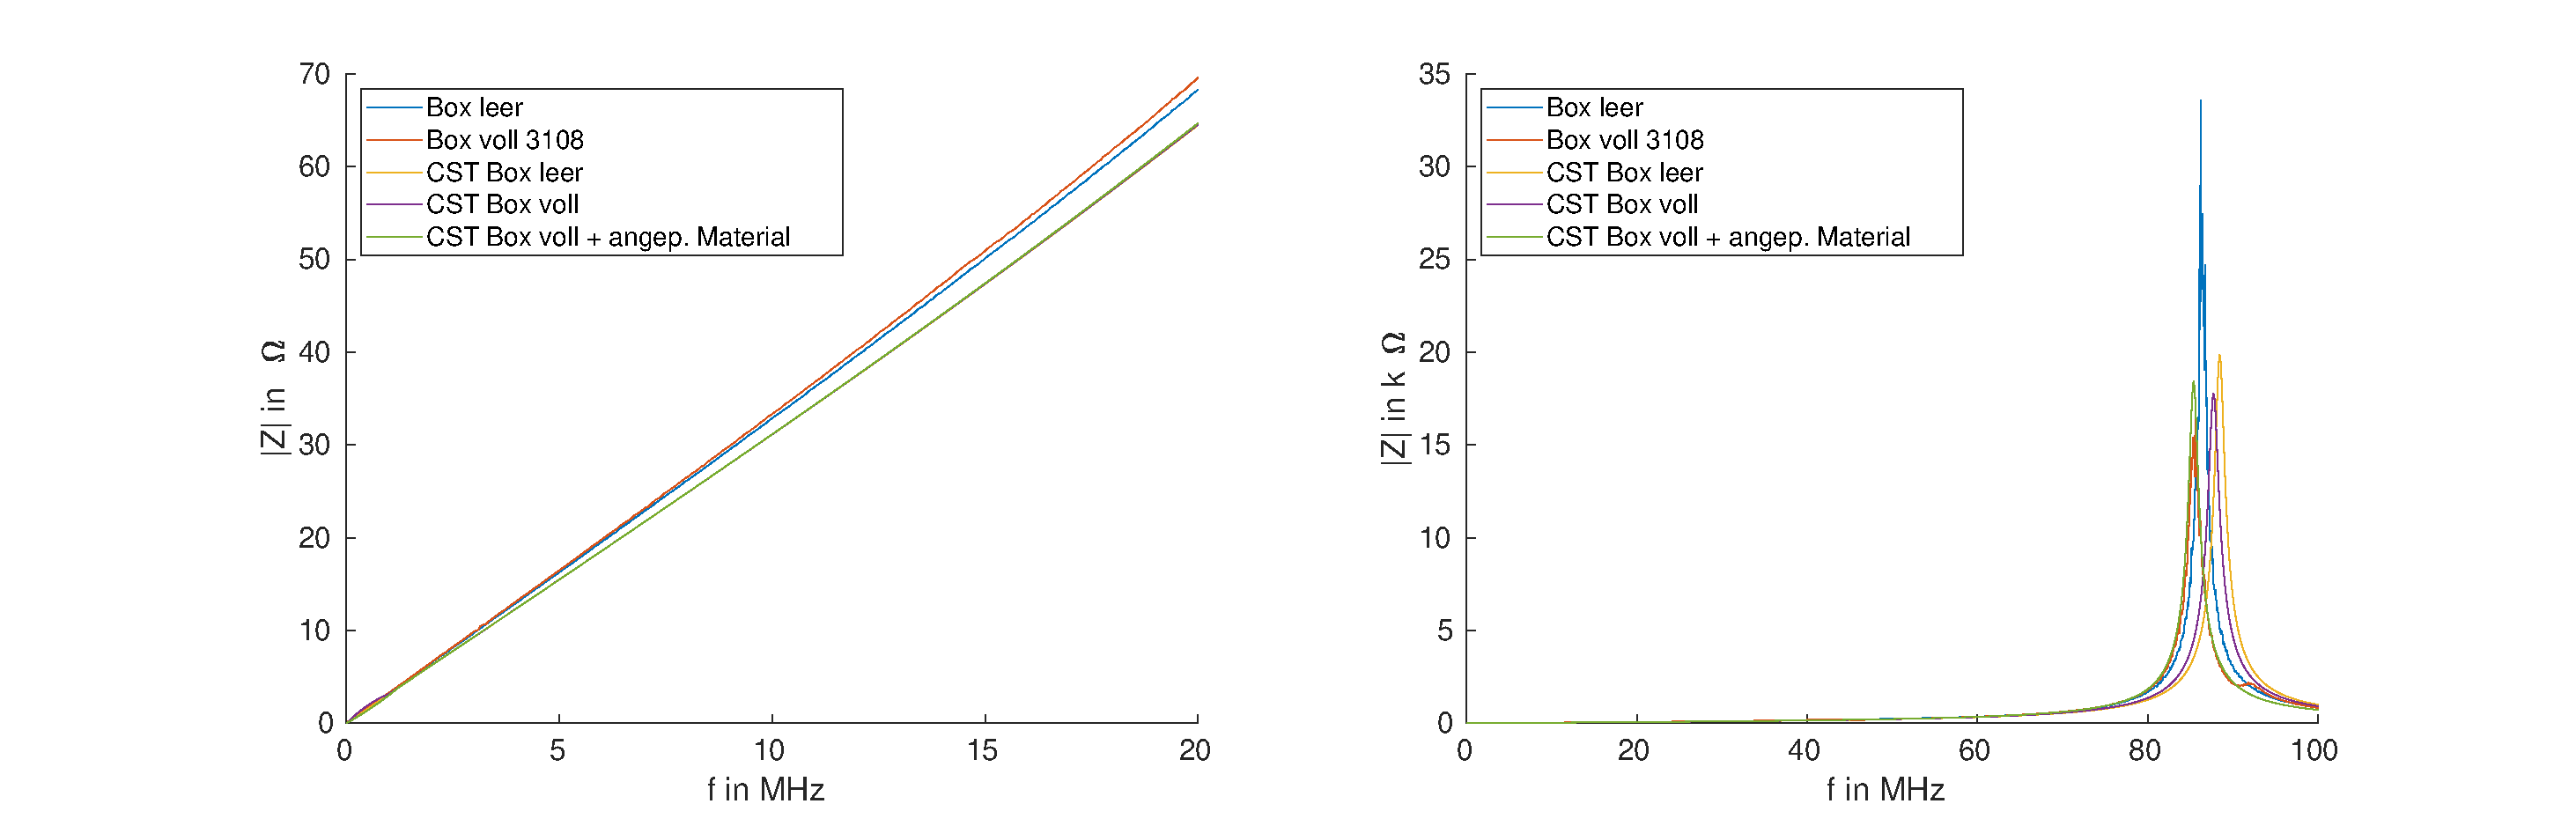
\includegraphics[width=\textwidth]{measurement_simulation_emptybox}
	\caption{Gegen\"uberstellung der Simulation der Box mit Halterung aus Kreuz und Polygon zur entsprechenden Messung.}
	\label{fig:boxpolycross}
\end{figure}
\par
Als n\"achstes in das Modell mit eingesetztem Ringkern zu evalieren. Dazu wird der Ringkern f\"ur die Simulation auf der Position um den Trovidur Ring gelegt, um die reale Box genau abzubilden. Der Aufbau ist in Abbildung~\ref{fig:RKFeRingCST} gezeigt worden. Auch hierbei wird wieder die gemessene Impedanz an der Einkopplung direkt mit der Impedanz aus der Simulation gegen\"ubergestellt. Diese Auswertung ist in Abbildung~\ref{fig:boxpolycrossrk} zu sehen.



\newpage



\begin{figure}[htb]
	\centering
	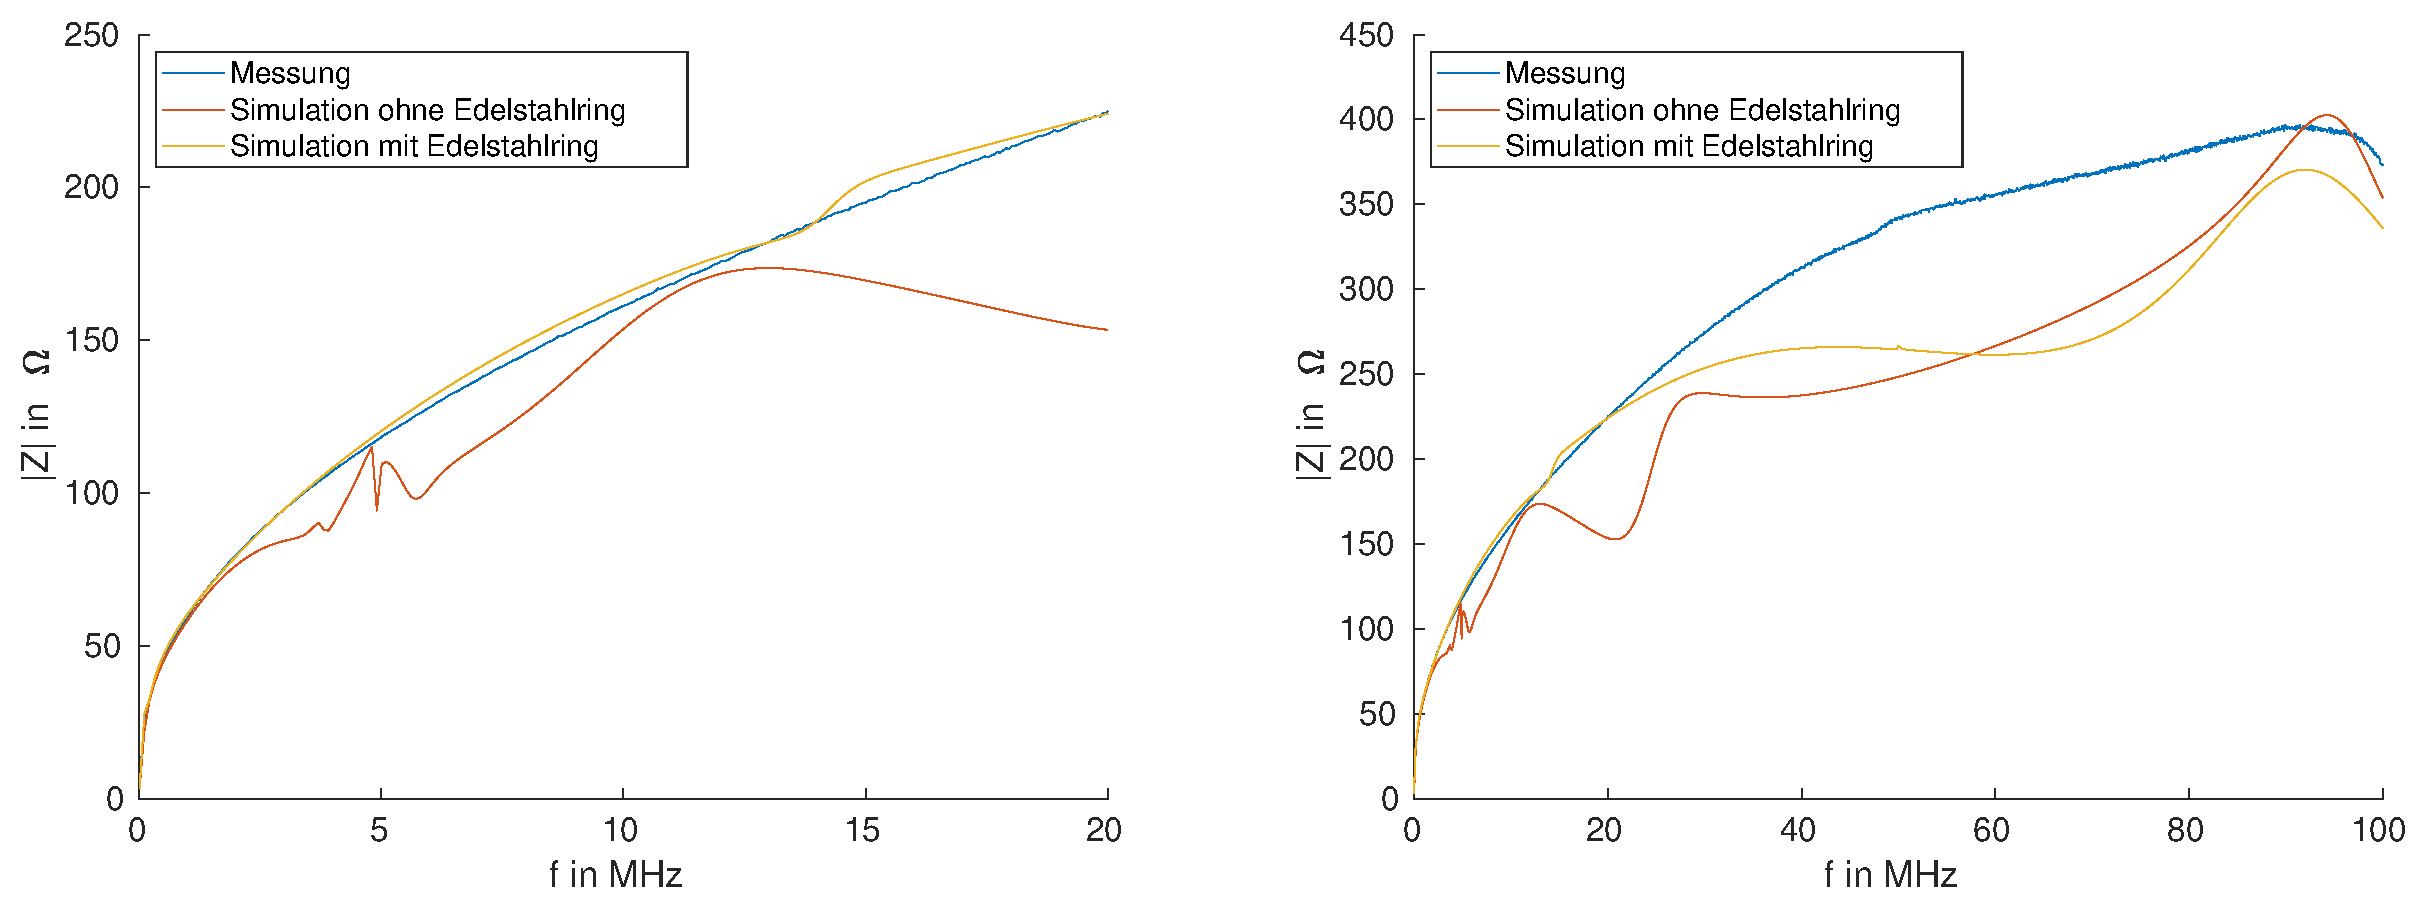
\includegraphics[width=\textwidth]{Zges_RK_SimMeas}
	\caption{Gegen\"uberstellung der gemessenen, mit der simulierten Ringkernimpedanz ohne Kurzschl\"usse}
	\label{fig:boxpolycrossrk}
\end{figure}
\par
Die Simulation zeigt auch nach mehrfacher Wiederholung mit verschiedenen Einstellungen eine starke Welligkeit. Die Konvergenz gegen die gemessenen Werte ist in dieser Anordnung daher schwer zu bewerten. 
\todo[inline,color=red!30]{Etwas mehr ausarbeiten wenn mir was einf\"allt}.  
% \par
% Die Gegen\"uberstellung wird f\"ur alle in Abschnitt~\ref{sec:testbox} genannten Kurzschlussanordnungen in gleicher Form durchgef\"uhrt.
% Es zeigt sich schnell, dass insbesondere im niedrigen Frequenzbereich eine sehr geringe Abweichung zu erkennen ist. Die Mittlere Abweichung zwischen Simulation und Messung liegt unterhalb von $\SI{20}{\mega\hertz}$ bei nur 

% \todo[inline,color=red!30]{wert und ggf Rechnung einf\"ugen}.  
\par
Auch die Kurzschlussmessungen wurden mit der Simulation gegen\"ubergestellt. Zun\"achst wird die Anordnung mit nur einem Kurzschluss in betrachtet. Insbesondere im Bereich bis $\SI{50}{\mega\hertz}$ ist eine hohe \"Ubereinstimmung zu sehen. Lediglich im h\"oheren Frequenzbereich, nahe der Resonanz, weichen Messung und Simulation voneinander ab. Abbildung~\ref{fig:boxpolycrossrk1ks} zeigt die Gegen\"uberstellung.
\begin{figure}[htb]
	\centering
	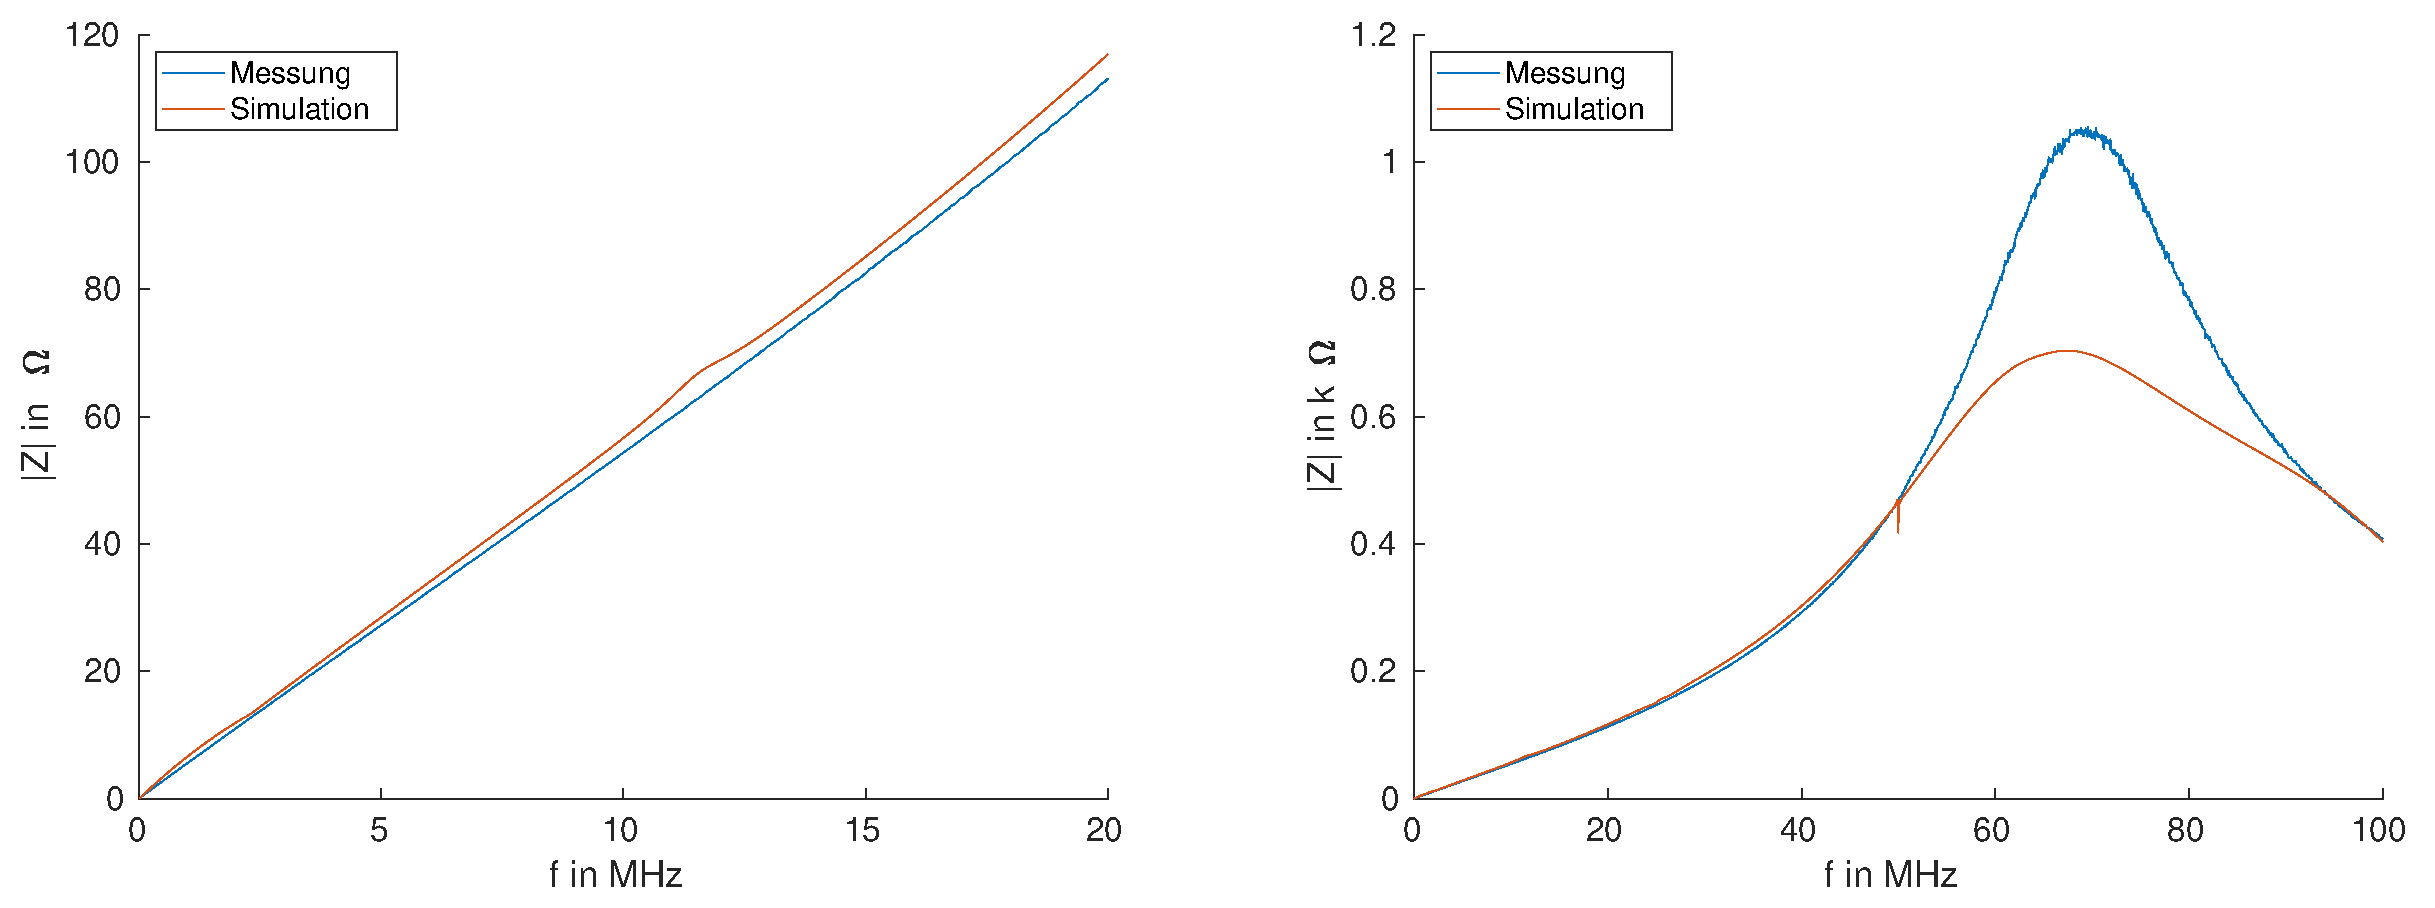
\includegraphics[width=\textwidth]{Z_ges_1KS_SimMeas}
	\caption{Gegen\"uberstellung der gemessenen, mit der simulierten Ringkernimpedanz f\"ur einen Kurzschluss.}
	\label{fig:boxpolycrossrk1ks}
\end{figure}



\newpage



Die Simulation der weiteren Kurzschl\"ussanordnungen zeigt, dass die Simulation bei zunehmender Anzahl an Kurzschl\"ussen etwas st\"arker von der Messung abweicht, als bei wenigen Kurzschl\"ussen. Abbildung~\ref{fig:boxpolycrossrk7ks} zeigt diesen Effekt beispielhaft f\"ur eine Anzahl von sieben Kurzschl\"ussen.
\begin{figure}[htb]
	\centering
	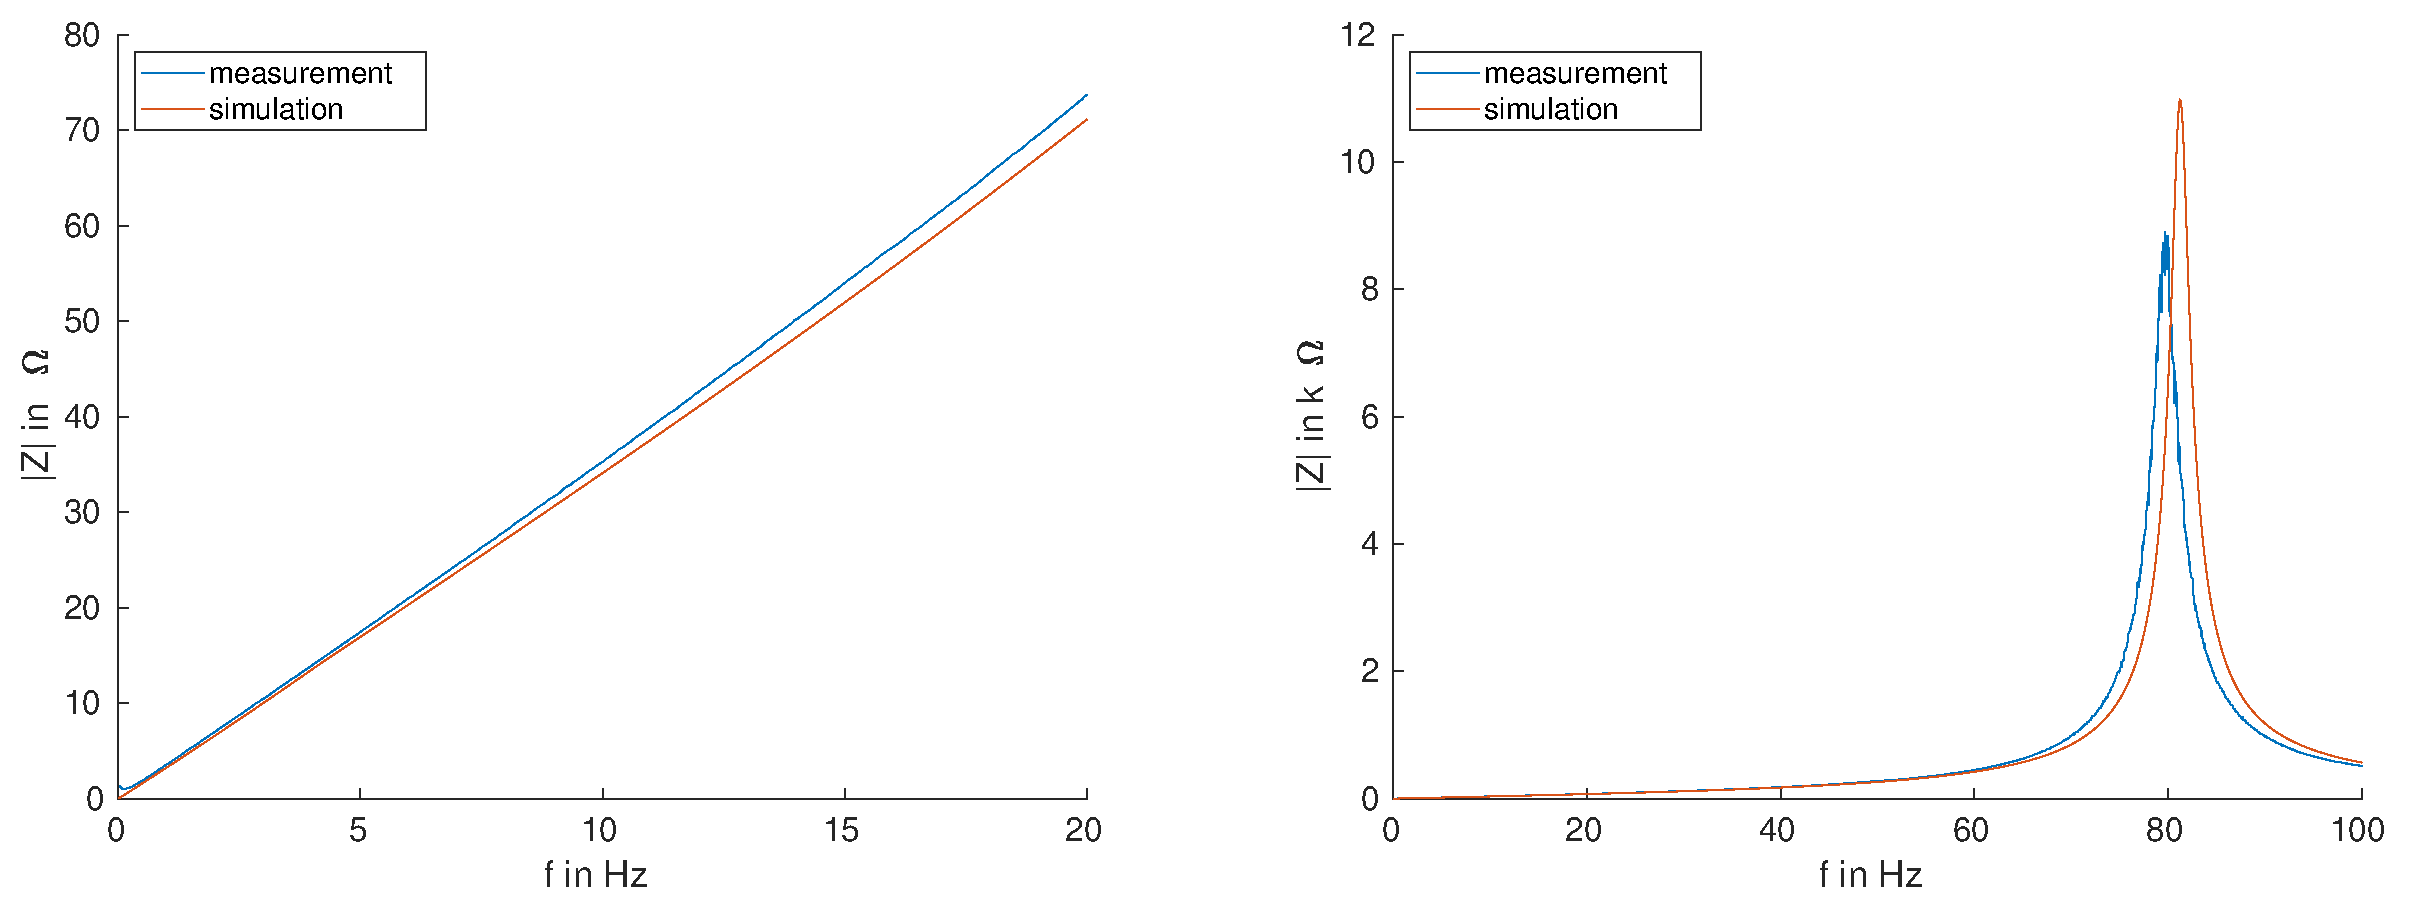
\includegraphics[width=\textwidth]{Z_ges_7KS_SimMeas}
	\caption{Gegen\"uberstellung der gemessenen, mit der simulierten Ringkernimpedanz f\"ur eine Anzahl von sieben Kurzschl\"ussen}
	\label{fig:boxpolycrossrk7ks}
\end{figure}
\par
Eine m\"ogliche Erkl\"arung daf\"ur w\"are, dass die simulierten Kurzschl\"usse idealere Materialeigenschaften, bessere Kontaktierung sowie eine h\"ohere Formsicherheit aufweisen, als es das Kupfer und die Verschraubung in der Realit\"at liefern k\"onnen. Die Gegen\"uberstellung aller Kurzschlussanordnungen in Simulation und Messung sind in Anhang~\ref{sec:simmesskomplett} abgebildet.


\section{Auswertung der Kurzschlussanordnungen}
Nachdem die Messungen, sowie die Simulationen gegeneinander abgeglichen sind, kann die Auswertung der Kurzschlussversuche begonnen werden. Dazu wird nur die reine Ringkernimpedanz r\"uckgerechnet. Analog zum in Abschnitt~\ref{sec:ringkern} beschriebenen vorgehen, wird auch hierzu die Impedanz $Z_{rk}$ aus der gemessenen Impedanz $Z_{ges}$ nach Gleichung~\ref{eq:Zrk} herausgerechnet. Somit l\"asst sich isoliert betrachten, welcher Anteil der Ringkernimpedanz nach dem zuf\"ugen der Kurzschl\"usse noch als Rest verbleibt. Gegen\"ubergestellt werden dazu die in Unterkapitel~\ref{sec:shorts} angef\"uhrten Variationsparameter.
\par
Die maximale realtive Abweichung $a_{max}$ wird f\"ur einen Variationsparameter  nach Gleichung~\ref{eq:maxdiff} berechnet.
\begin{equation}
	\frac{Z_{max}(f) - Z_{min}(f)}{Z_{rk}(f)} = a_{max}(f)
	\label{eq:maxdiff}
\end{equation}
\par
Dabei entspricht $Z_{max}$ der h\"ochsten gemessenen Impedanz unter \"Anderung des Variationsparameters und $Z_{min}$ der niedrigsten. $Z_{rk}$ bezeichnet die Impedanz des Rinkerns ohne Kurzschl\"usse. Um die relative Abweichung $a_{percent}$ in Prozent zu erhalten, wird die relative Abweichung $a_{max}$ nach Gleichung~\ref{eq:maxdiffpercent} mit 100 multipliziert.
\begin{equation}
	\frac{Z_{max}(f) - Z_{min}(f)}{Z_{rk}(f)}\cdot 100 = a_{percent}(f)
	\label{eq:maxdiffpercent}
\end{equation}


\subsection{Anzahl der Kurzschl\"usse}
Um den Einfluss verschiedener Anzahlen an Kurzschl\"ussen zu analysieren werden ein bis acht identische Kurzschl\"usse in der Testbox montiert. Abbildung~\ref{fig:ringcorenumberCST} zeigt die Positionen der montierten Kurzschl\"usse.
\begin{figure}[htb]
	\centering
	\subfloat{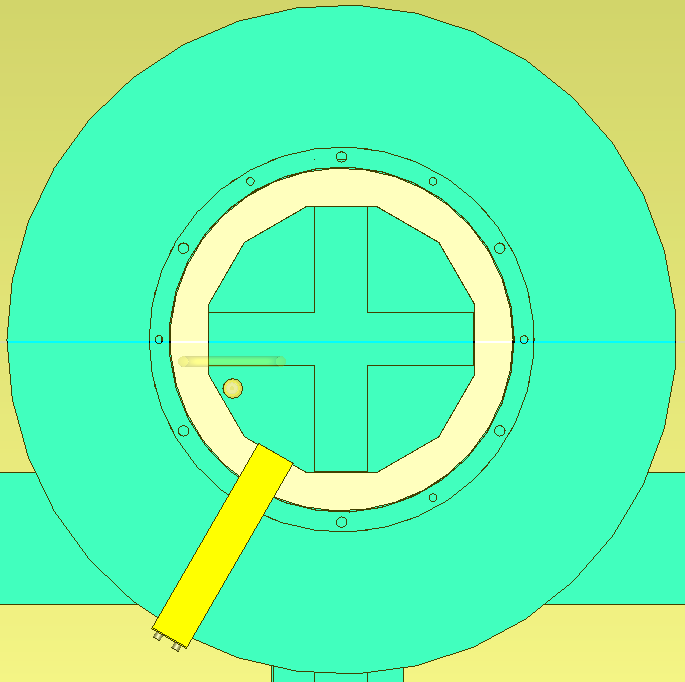
\includegraphics[height=0.24\textwidth]{1ksb30}}
	\hspace{0.0065\textwidth}
	\subfloat{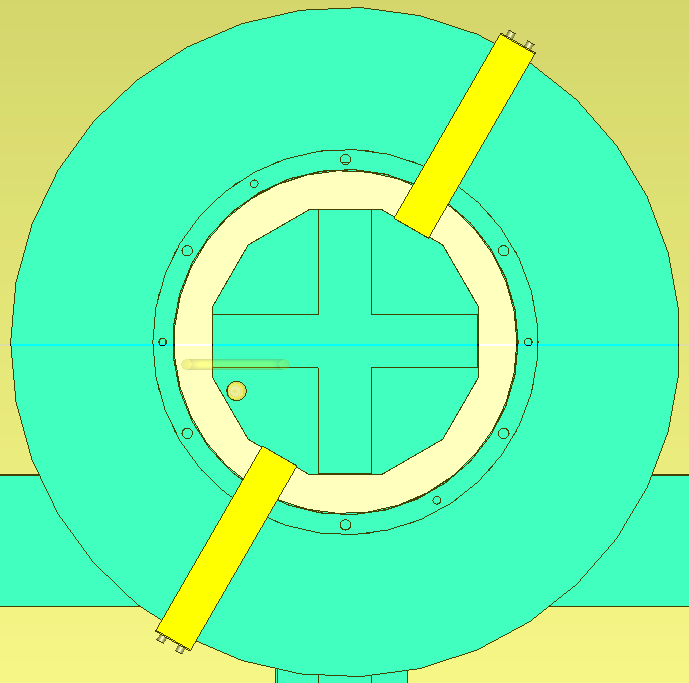
\includegraphics[height=0.24\textwidth]{2ksb30}}
	\hspace{0.0065\textwidth}
	\subfloat{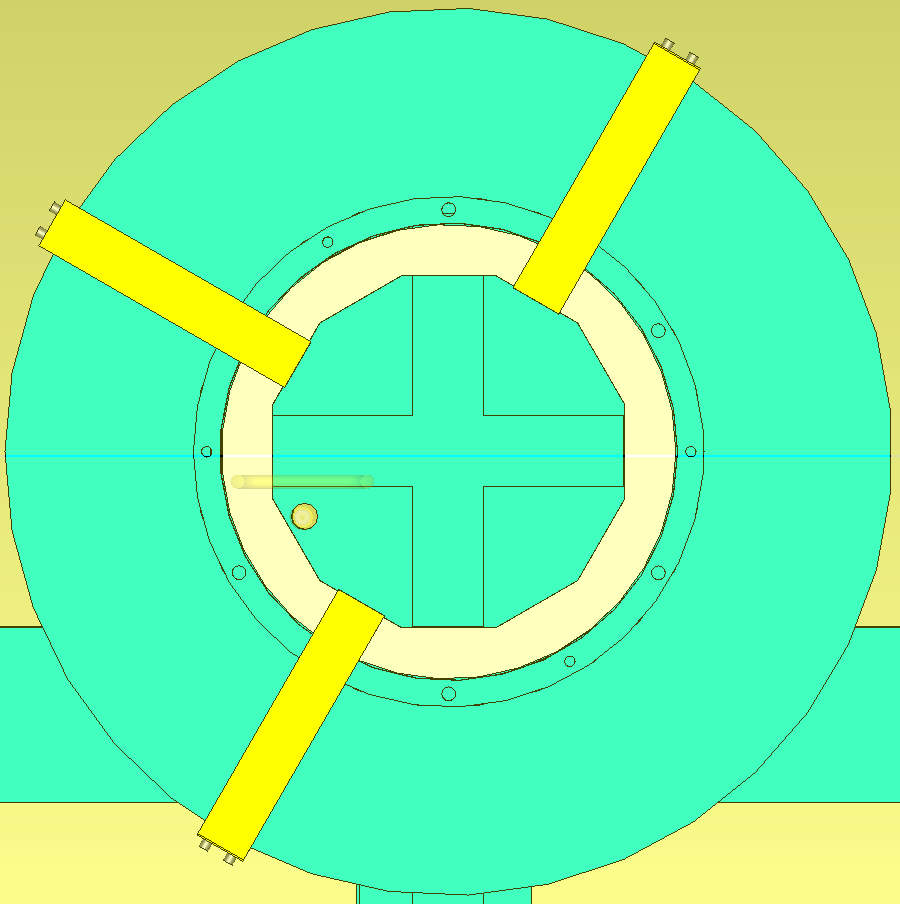
\includegraphics[height=0.24\textwidth]{3ksb30}}
	\hspace{0.0065\textwidth}
	\subfloat{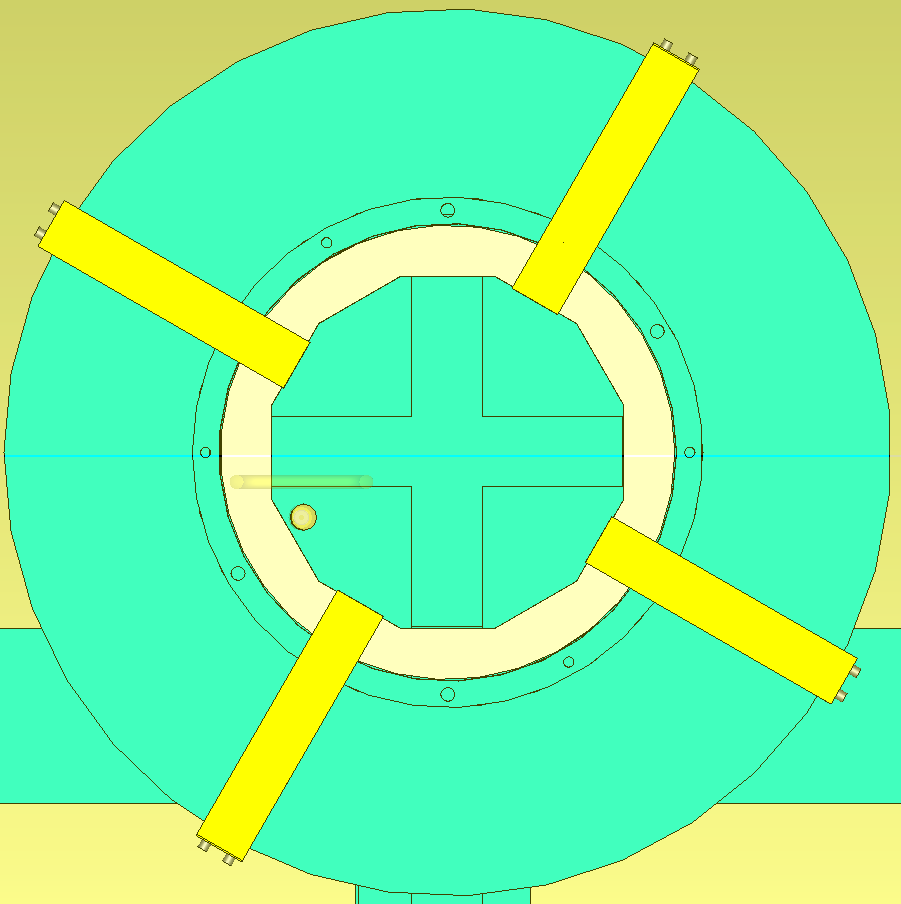
\includegraphics[height=0.24\textwidth]{4ksb30}}
	\\
	\subfloat{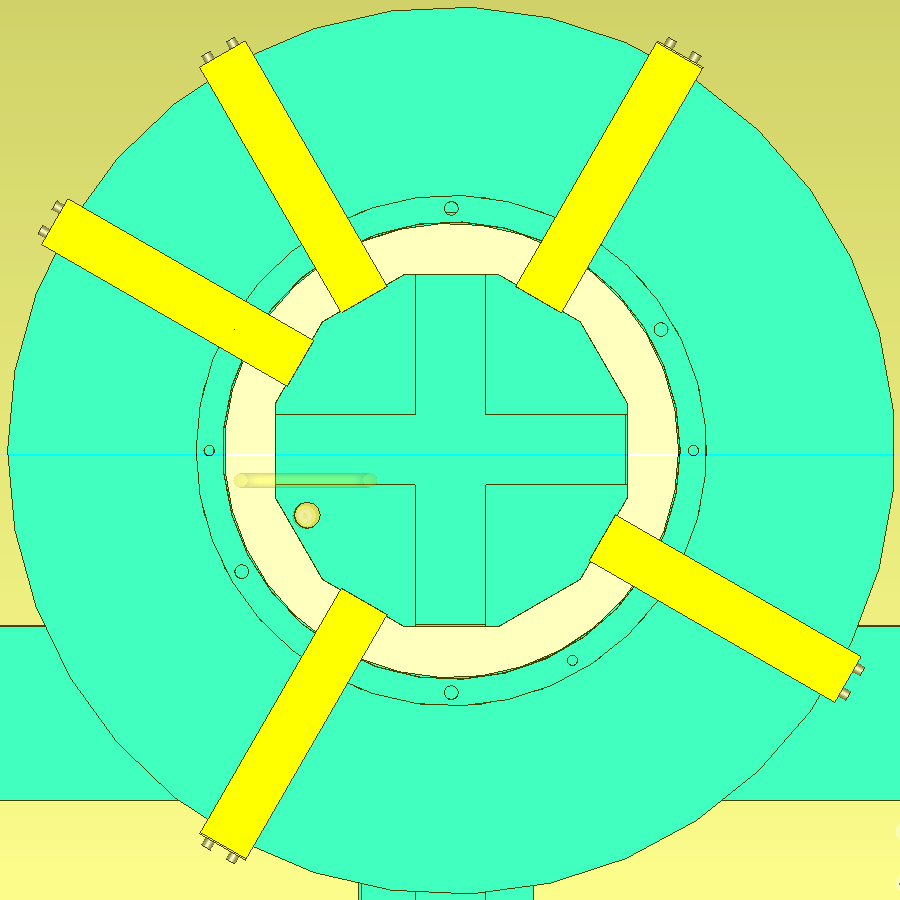
\includegraphics[height=0.24\textwidth]{5ksb30}}
	\hspace{0.0065\textwidth}
	\subfloat{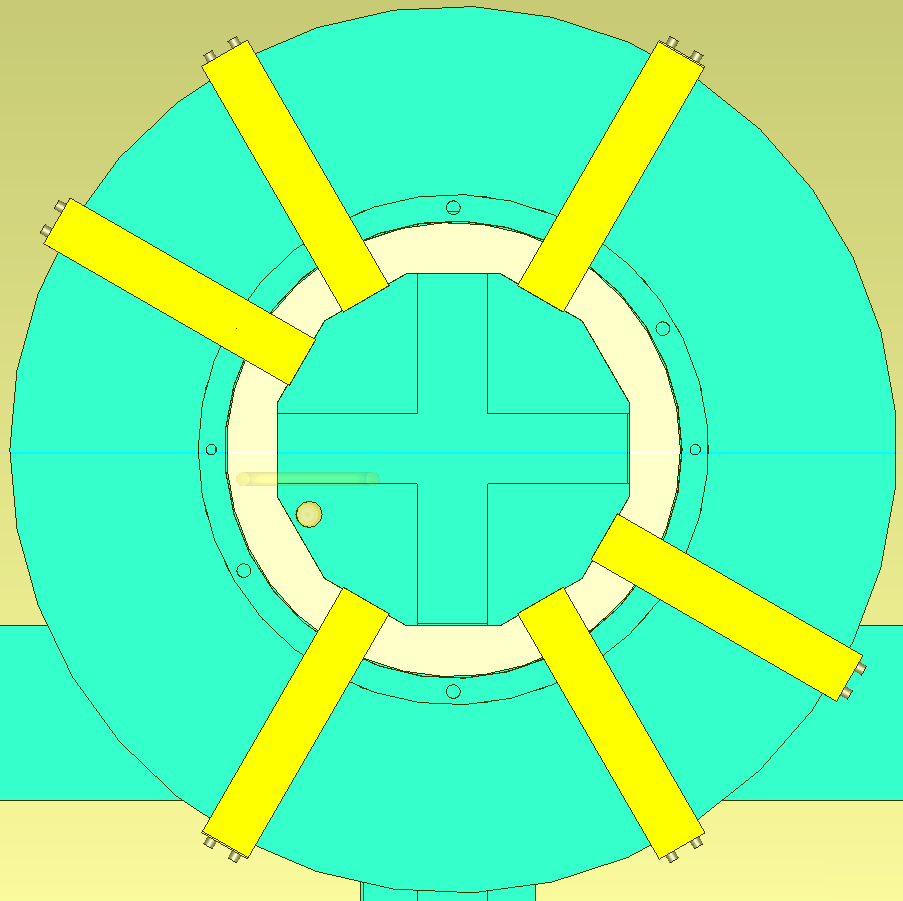
\includegraphics[height=0.24\textwidth]{6ksb30}}
	\hspace{0.0065\textwidth}
	\subfloat{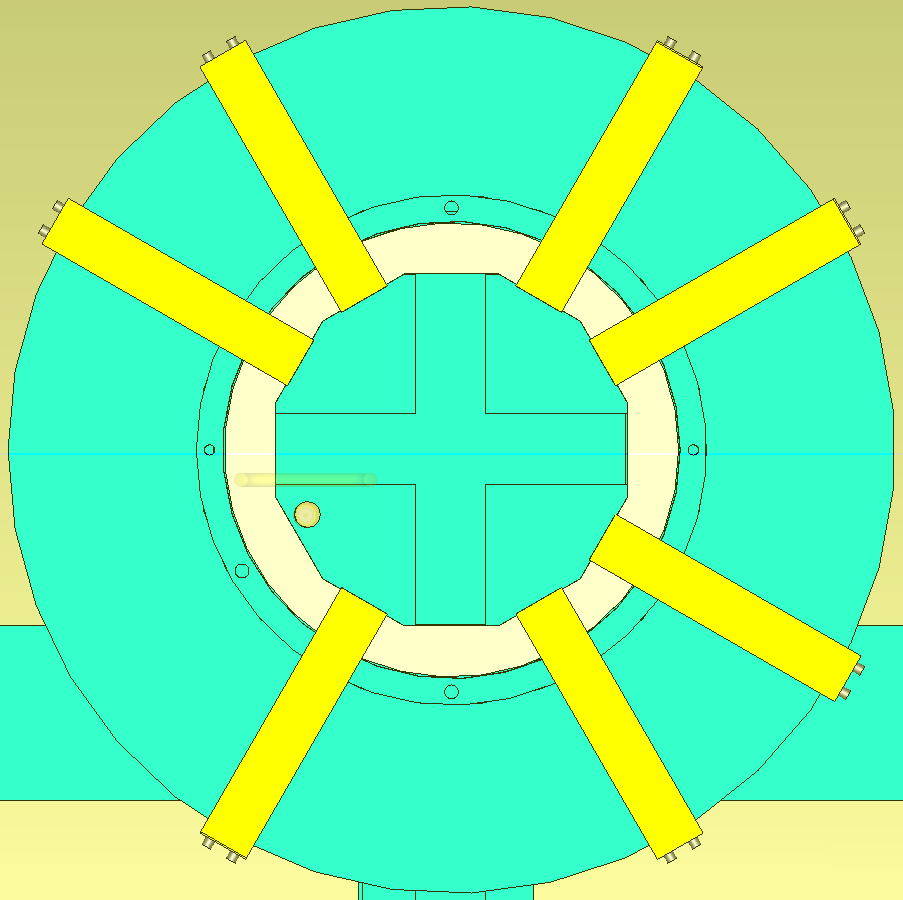
\includegraphics[height=0.24\textwidth]{7ksb30}}
	\hspace{0.0065\textwidth}
	\subfloat{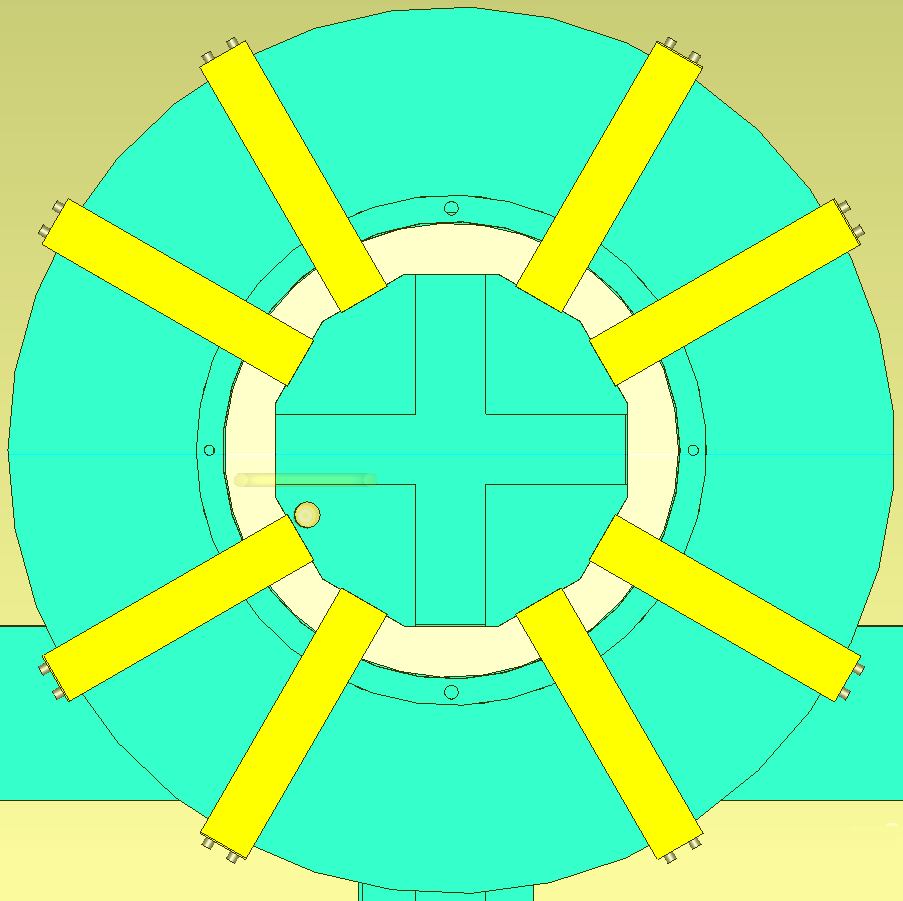
\includegraphics[height=0.24\textwidth]{8ksb30}}
	\caption{Unterschiedliche Anzahlen an montierten Kurzschl\"ussen an verschiedenen Positionen.}
	\label{fig:ringcorenumberCST}
\end{figure}
\par
% \todo[inline,color=red!30]{Erkl\"aren warum 8KS bei der Auswertung nicht mehr auftaucht}  
Die achte Kurzschlusschiene, welche in Grafik~\ref{fig:ringcorenumberCST} zu sehen ist, konnte bei der endg\"ultigen Auswertung nicht ber\"ucksichtigt werden. Dieser Kurzschluss liegt sehr nah am Einkopplungsrohr, sodass ein direkter Kontakt dazu besteht. F\"ugt man einen Abstandshalter aus Schaumstoff zu, so wird das die Einkopplung etwas nach oben gebogen. Die Messung liefert daher verf\"alschte Ergebnisse, welche deutlich st\"arker von der Simulation abweichen, als bei anderen Messungen. Auch dieses Verhalten ist in Anhang~\ref{sec:simmesskomplett} abgebildet. F\"ur die endg\"ultige Auswertung wurden folglich nur 1-7 Kurzschl\"usse betrachtet. Die resultierende Ringkernimpedanz f\"ur die einzelnen Kurzschlussanordnungen ist in Abbildung~\ref{fig:ringcorenumber} \"uber der Frequenz aufgetragen.


\newpage



\begin{figure}[htb]
	\centering
	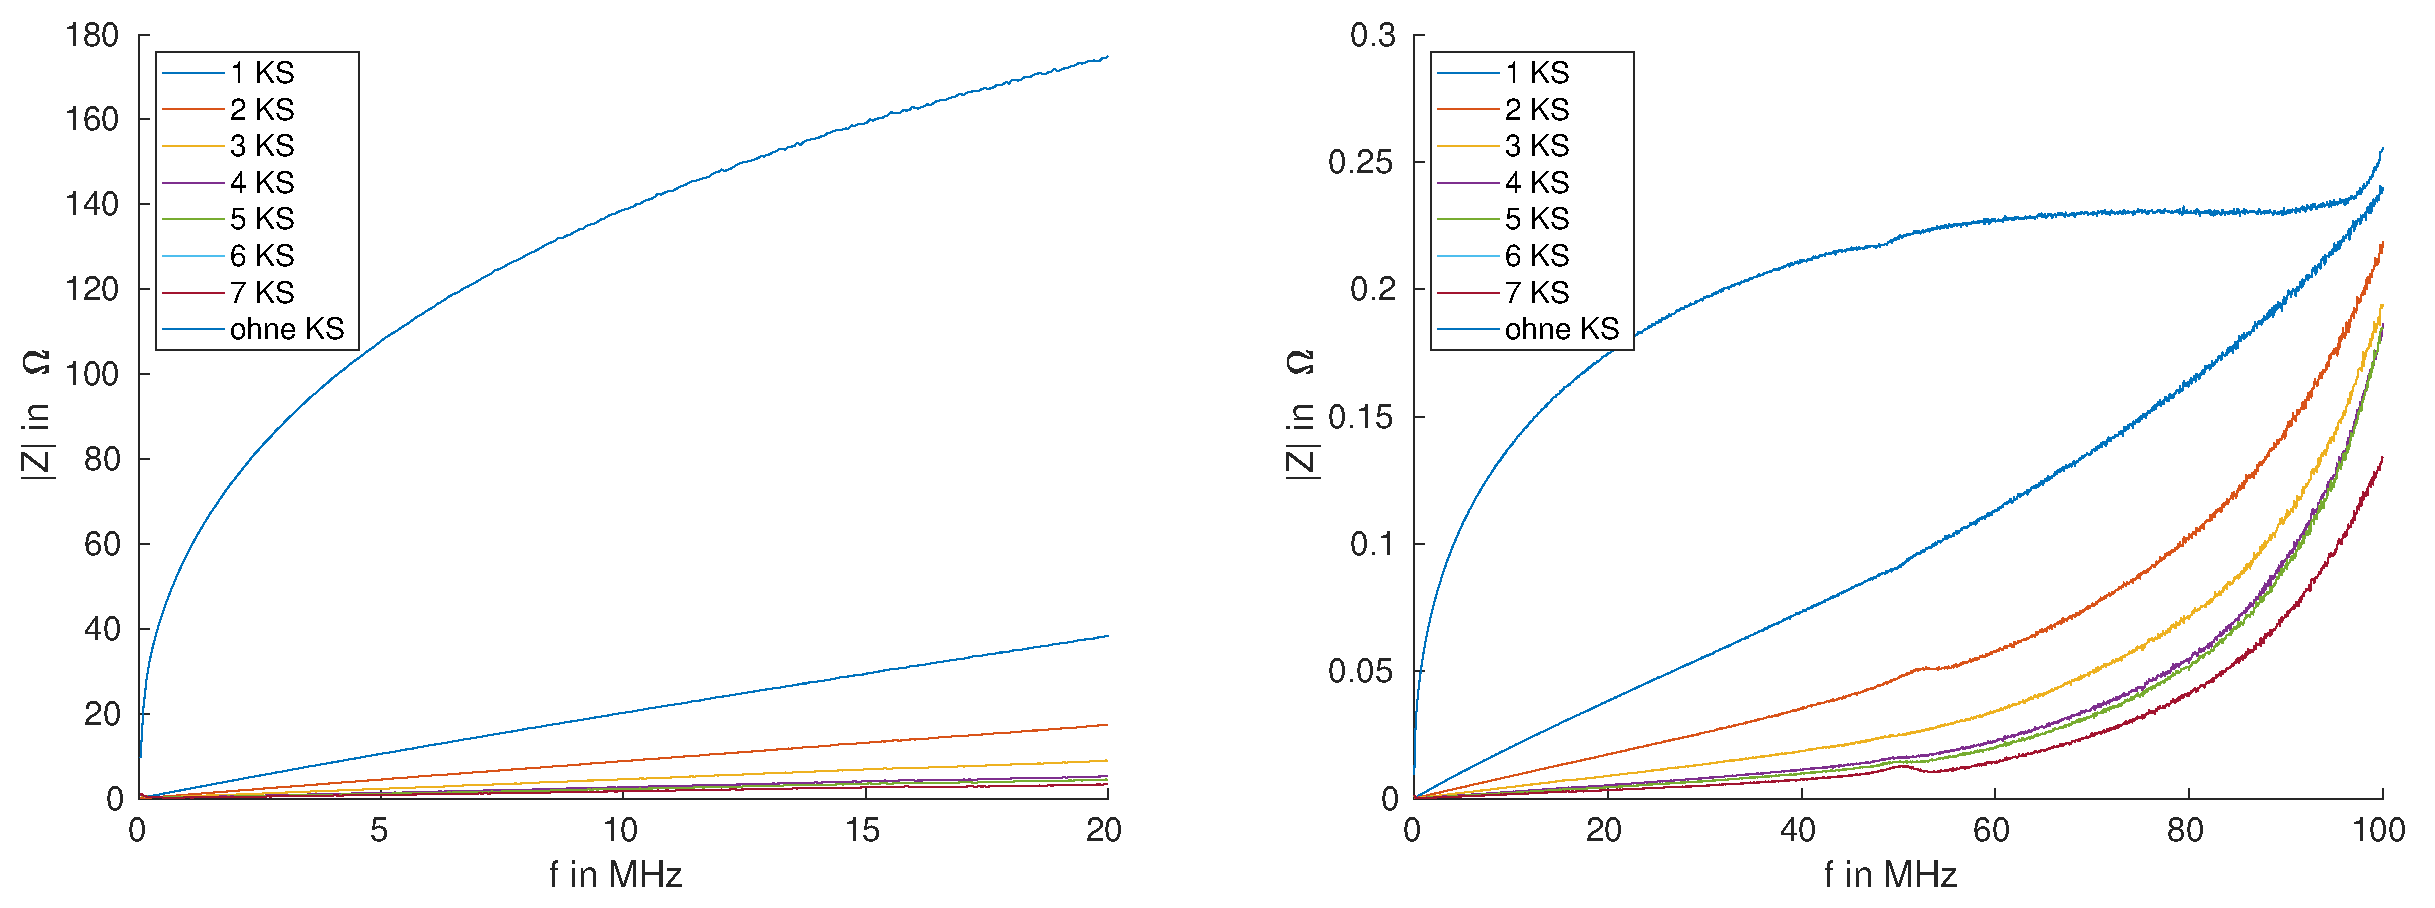
\includegraphics[width=\textwidth]{impedance_numberKS_ringcore}
	\caption{Gegen\"uberstellung der Ringkernimpedanz \"uber der Frequenz f\"ur verschiedene Anzahlen an Kurzschl\"ussen}
	\label{fig:ringcorenumber}
\end{figure}
\par
Es f\"allt auf, dass der gr\"o\ss{}te Sprung zwischen null und einem Kurzschluss liegt. Das bedeutet, dass die Montage weiterer Kurzschl\"usse mit zunehmender Anzahl weniger effektiv ist. Um das zu verdeutlichen wird eine weitere Gegen\"uberstellung angesetzt, bei der eine bestimmte Frequenz fixiert wird, und die Ringkernimpedanz \"uber der Anzahl an Kurzschl\"ussen aufgetragen ist. Die fixierten Frequenzen liegen dabei bei 5, 10 und $\SI{20}{\mega\hertz}$, da insbesondere der niedrigere Frequenzbereich f\"ur den Beschleunigerbetrieb von Relevanz ist~\citep{frey2015status}. Die Gegen\"uberstellung ist in Abbildung~\ref{fig:ringcorenumber20} aufgetragen.
\begin{figure}[htb]
	\centering
	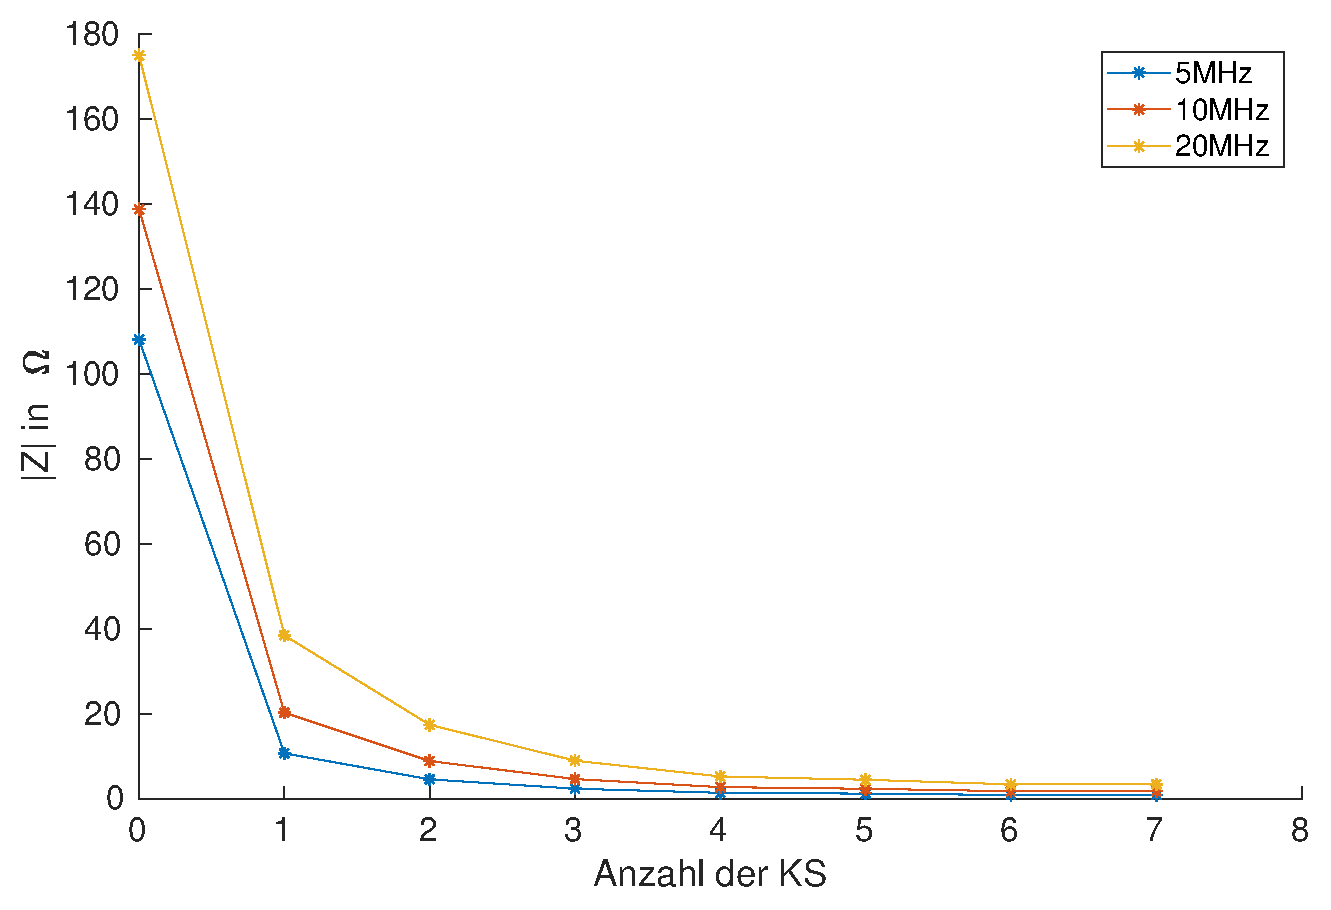
\includegraphics[width=0.5\textwidth]{RK_Impedanz_numberKS_frequenz}
	\caption{Gegen\"uberstellung der Ringkernimpedanz mit verschiedenen Anzahlen an Kurzschl\"ussen bei 5, 10 und $\SI{20}{\mega\hertz}$.}
	\label{fig:ringcorenumber20}
\end{figure}
\par
Der Effekt der Kurzschl\"usse wird mittels Gleichung~\ref{eq:maxdiffpercent} errechnet. Wird $Z_{max}$ auf den Wert $Z_{rk}(\SI{20}{\mega\hertz})$ gesetzt, also den Fall ohne Kurzschl\"usse und $Z_{min}$ auf $Z_{1KS}(\SI{20}{\mega\hertz})$, so ergibt sich eine prozentuale Verringerung der Impedanz nach Gleichung~\ref{eq:maxdiffpercentzeroone}.
\begin{equation}
	\frac{\SI{175,1145}{\Omega} - \SI{38,4525}{\Omega}}{\SI{175,1145}{\Omega}}\cdot 100 = \SI{78,042}{\%}
	\label{eq:maxdiffpercentzeroone}
\end{equation}
\par
Das hei\ss{}t ein Kurzschluss verringert die Impedanz des Ringkerns bereits um $\SI{78,042}{\%}$ verglichen mit der Impedanz ohne Kurzschluss. Wird hingegen $Z_{max}$ auf $Z_{1KS}(\SI{20}{\mega\hertz})$ und $Z_{min}$ zu $Z_{2KS}(\SI{20}{\mega\hertz})$ gesetzt, so ergibt sich nach Gleichung~\ref{eq:maxdiffpercentonetwo}.
\begin{equation}
	\frac{\SI{38,4525}{\Omega} - \SI{17,3717}{\Omega}}{\SI{175,1145}{\Omega}}\cdot 100 = \SI{12,038}{\%}
	\label{eq:maxdiffpercentonetwo}
\end{equation}
\par
Die Verringerung der Impedanz f\"allt also deutlich geringer aus, als noch beim Unterschied von Null zu einem Kurzschluss. Auch der Vergleich von einem zu sieben Kurzschl\"ussen, also mit $Z_{max}$ gleich $Z_{1KS}(\SI{20}{\mega\hertz})$ und $Z_{min}$ gleich $Z_{7KS}(\SI{20}{\mega\hertz})$ f\"allt mit der Abweichung nach Gleichung~\ref{eq:maxdiffpercentoneseven}
\begin{equation}
	\frac{\SI{38,4525}{\Omega} - \SI{3,3453}{\Omega}}{\SI{175,1145}{\Omega}}\cdot 100 = \SI{20,048}{\%}
	\label{eq:maxdiffpercentoneseven}
\end{equation}
\par
vergleichsweise geringer aus. Je nach Anforderung ist also zu \"uberlegen, ob ein Kurzschluss bereits eine ausreichende Reduktion der Impedanz erzeugt. Das ist insbesondere beim Einbau in die Kavit\"at von Relevanz, da eine Montage mehrerer Kurzschl\"usse einen nicht unerheblichen Aufwand mit sich zieht. 


\subsection{Breite der Kurzschl\"usse}
Die Breite der Kurzschl\"usse ist ein Parameter, welcher durch die Schienenartige Form der Kurzschl\"usse leicht zu variieren ist, da diese nur aus einem Blech geschnitten werden. Die Montierten Kurzschl\"usse verschiedener Breiten sind in Abbildung~\ref{fig:ringcorewidthCST} abgebildet.
\begin{figure}[htb]
	\centering.
	\subfloat[$\SI{20}{\milli\meter}$]{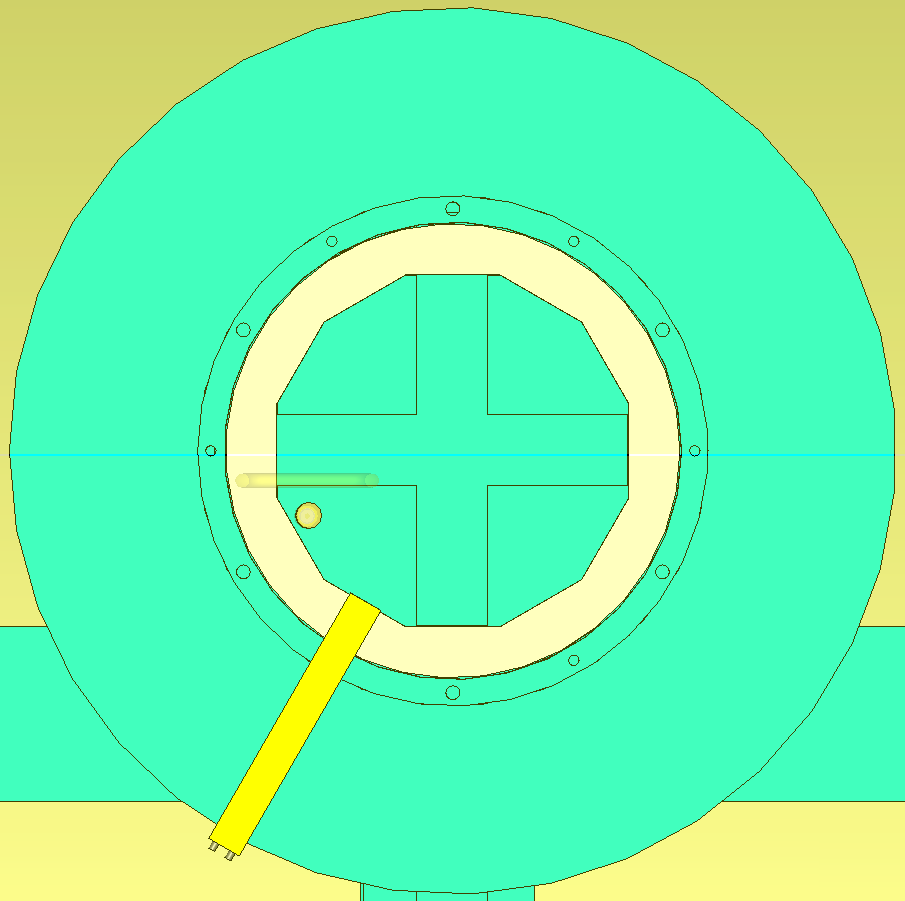
\includegraphics[height=0.3\textwidth]{1ksb20}}
	\hspace{0.02\textwidth}
	\subfloat[$\SI{30}{\milli\meter}$]{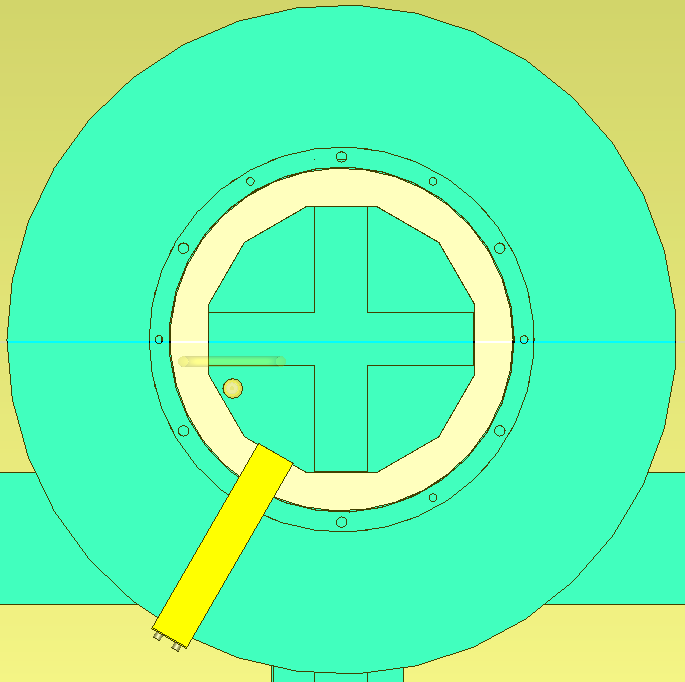
\includegraphics[height=0.3\textwidth]{1ksb30}}
	\hspace{0.02\textwidth}
	\subfloat[$\SI{50}{\milli\meter}$]{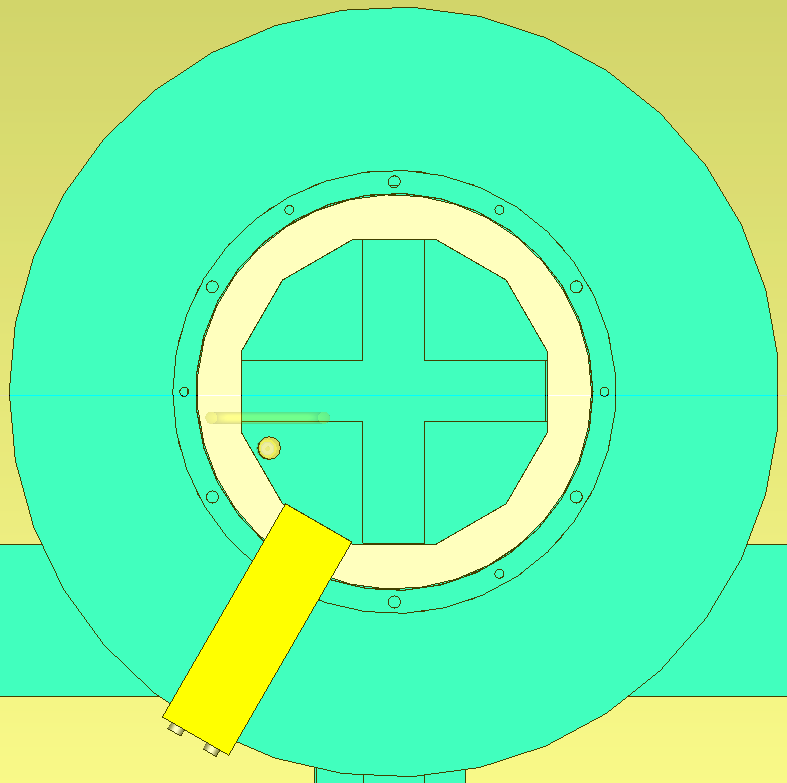
\includegraphics[height=0.3\textwidth]{1ksb50}}
	\caption{Jeweils ein montierter Kurzschluss mit verschiedenen Breiten.}
	\label{fig:ringcorewidthCST}
\end{figure}



\newpage



Da eine h\"ohere Anzahl an Kurzschl\"ussen eine verringerte Ringkernimpedanz als Ergebnis liefert, liegt die Vermutung nahe, dass auch breitere Kurzschl\"usse die Ringkernimpedanz weiter verringern k\"onnen. Die Gegen\"uberstellung der Ringkernimpedanz $Z_{rk}$ ist in Abbildung~\ref{fig:ringcorewidth} zu sehen.
\begin{figure}[htb]
	\centering
	\subfloat[1 Kurzschluss]{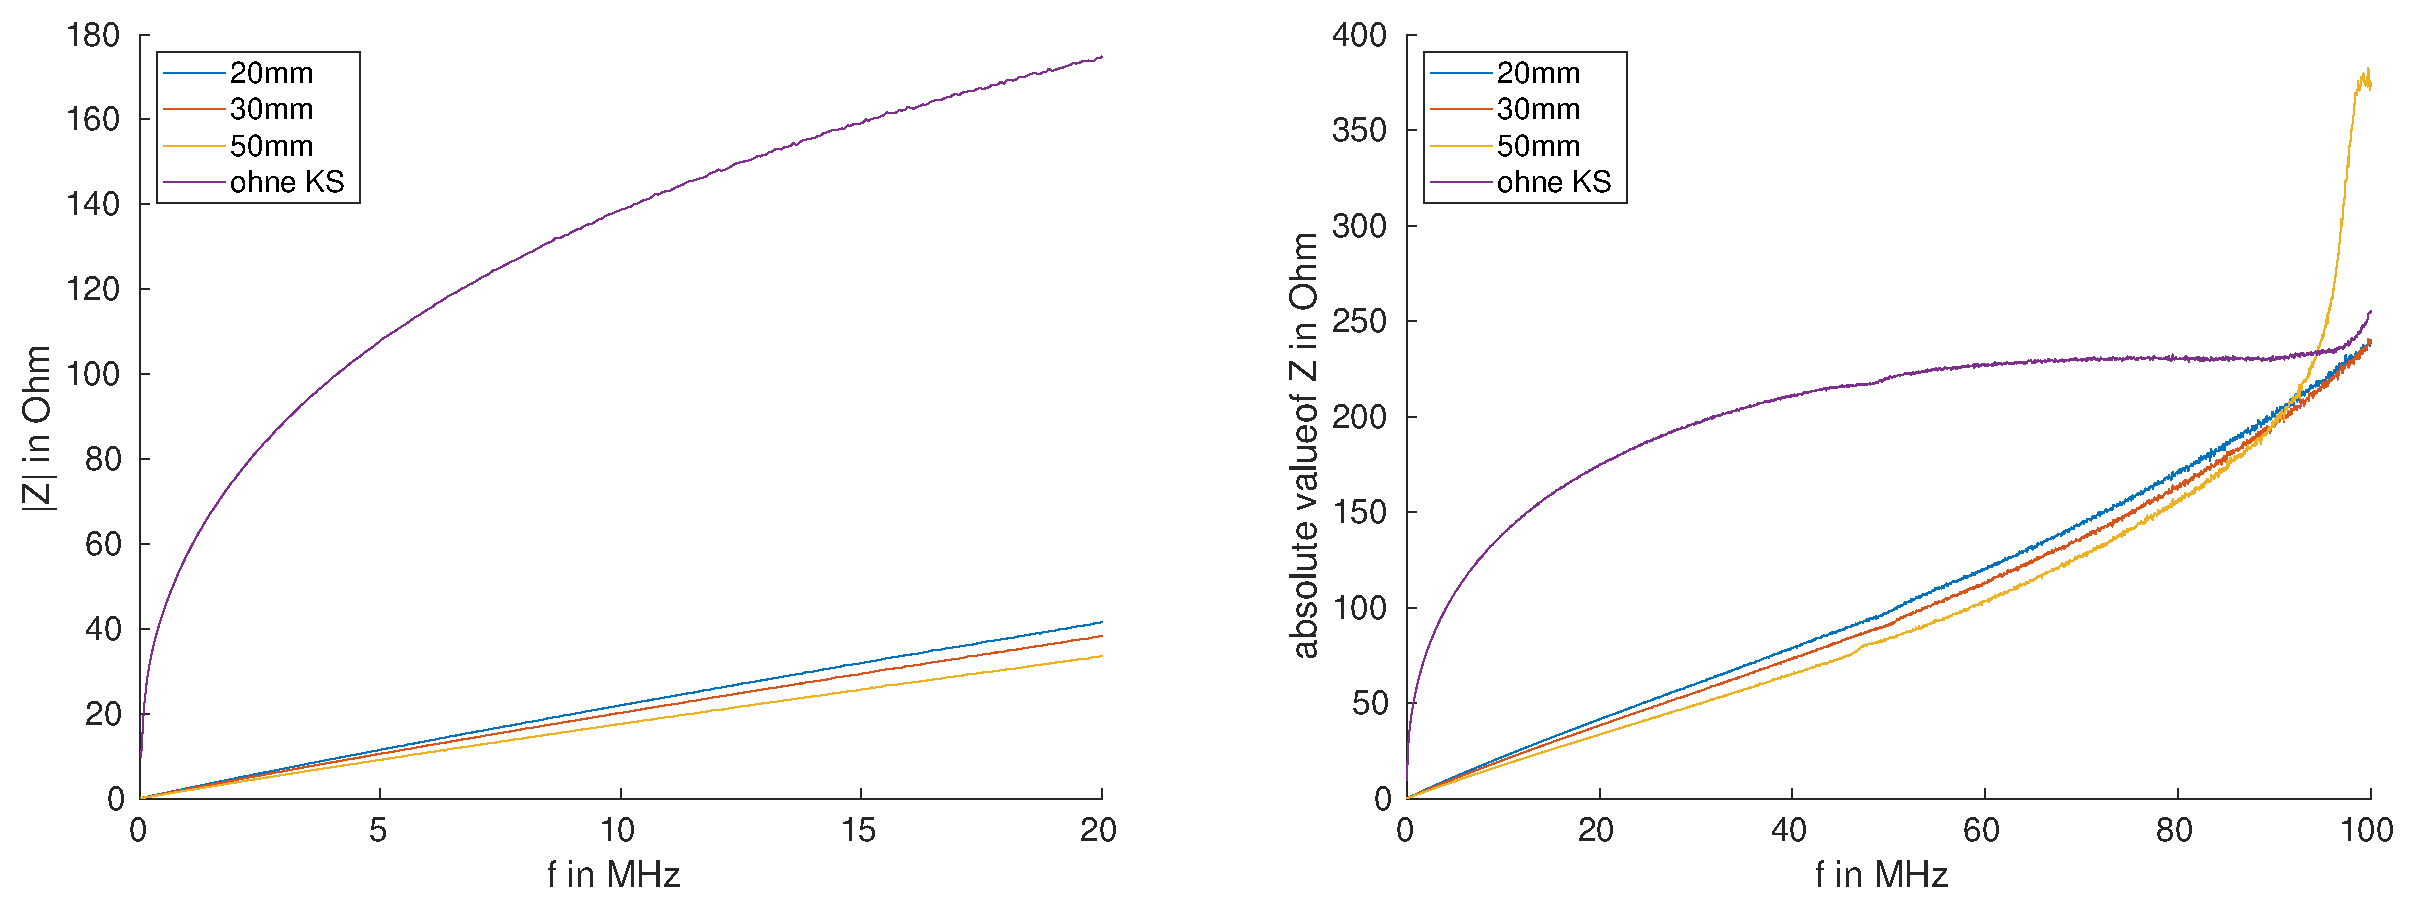
\includegraphics[width=\textwidth]{Z_RK_width_1KS}}
	\\
	\subfloat[2 Kurzschl\"usse]{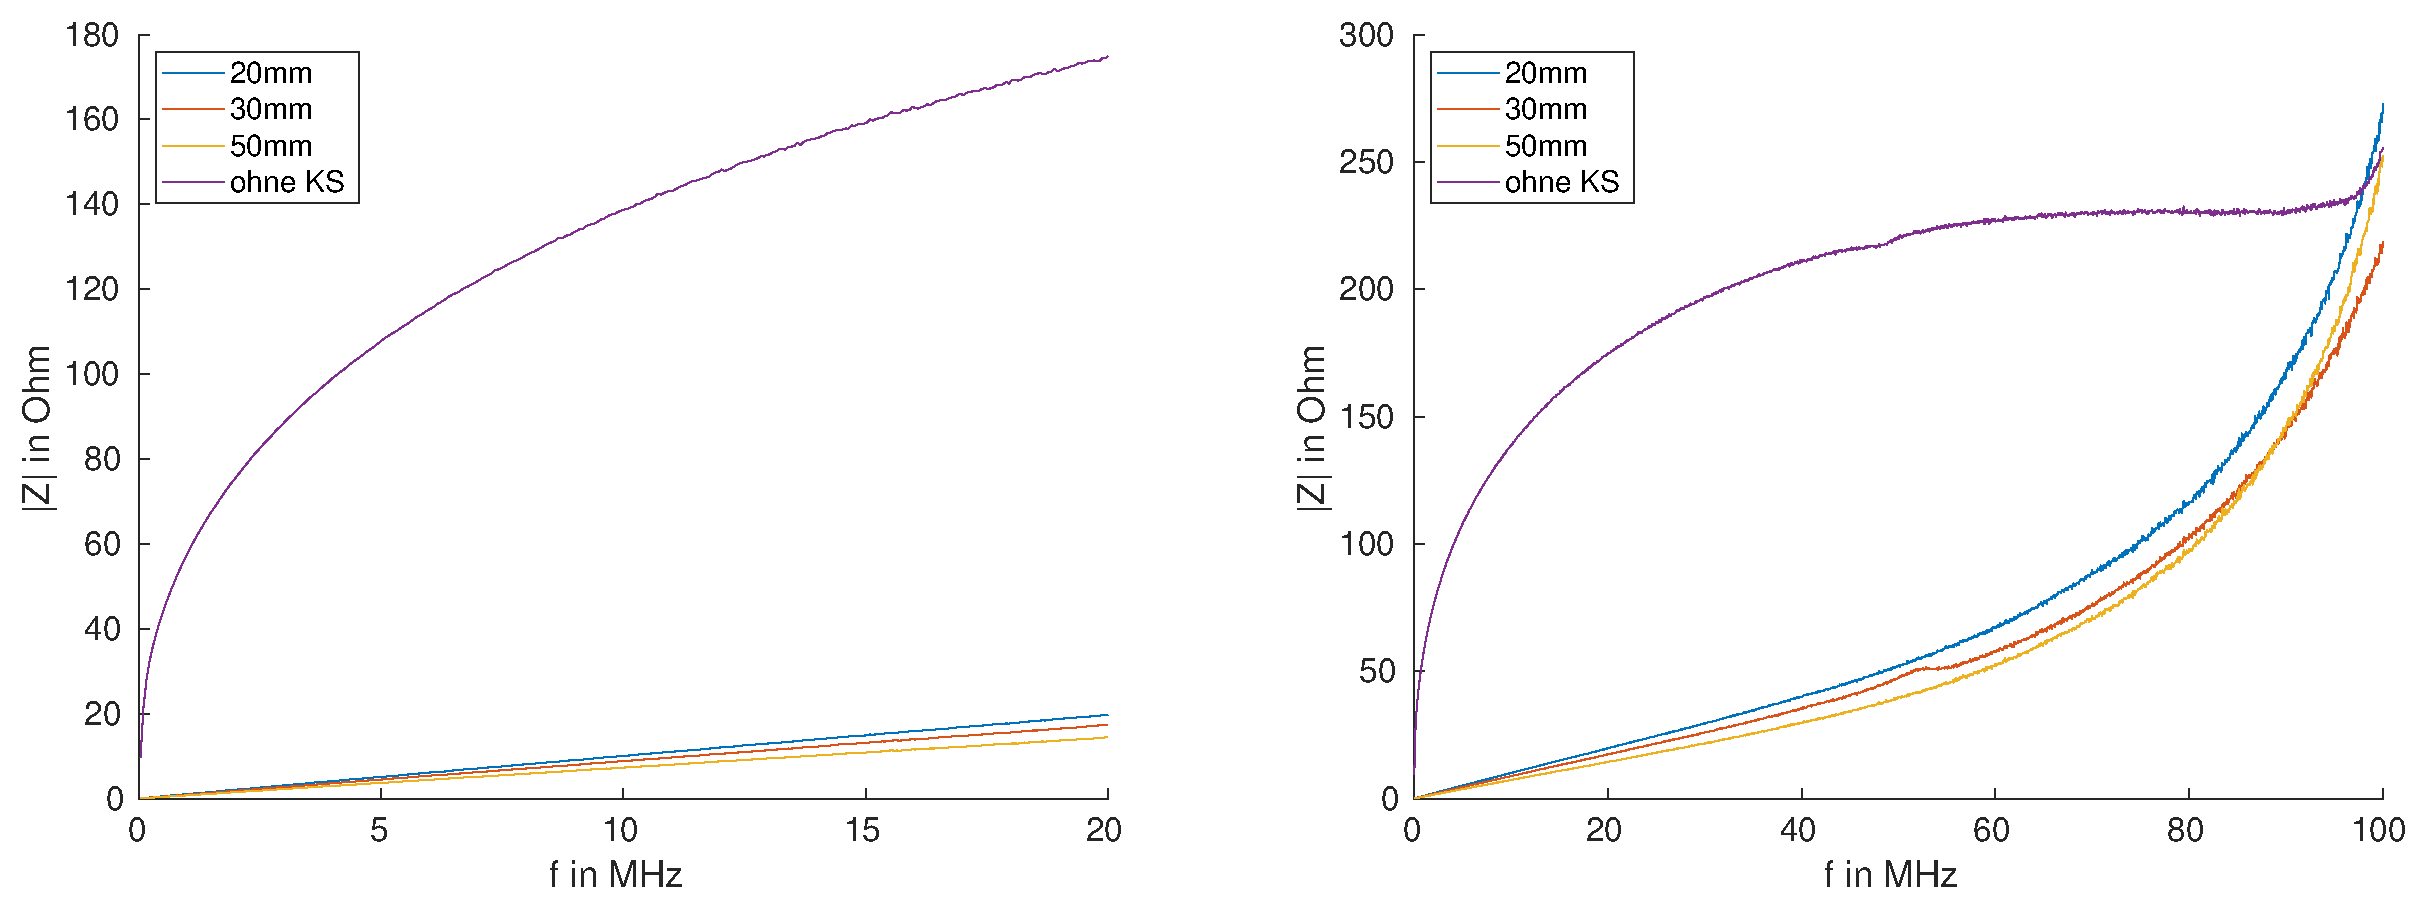
\includegraphics[width=\textwidth]{Z_RK_width_2KS}}
	\caption{Gegen\"uberstellung der Ringkernimpedanz f\"ur verschiedene Breiten der Kurzschl\"usse.}
	\label{fig:ringcorewidth}
\end{figure}
\par
Auch hier wird wieder ein genaueres Augenmerk auf den relevanten Frequenzbereich unterhalb von $\SI{20}{\mega\hertz}$ gelegt. Dazu werden die Frequenzen von 5, 10 und $\SI{20}{\mega\hertz}$ geplottet und jeweils die verschiedenen Breiten gegen\"ubergestellt. Abbildung~\ref{fig:ringcorewidth20} zeigt die genannte Gegen\"uberstellung.



\newpage



\begin{figure}[h]
	\centering
	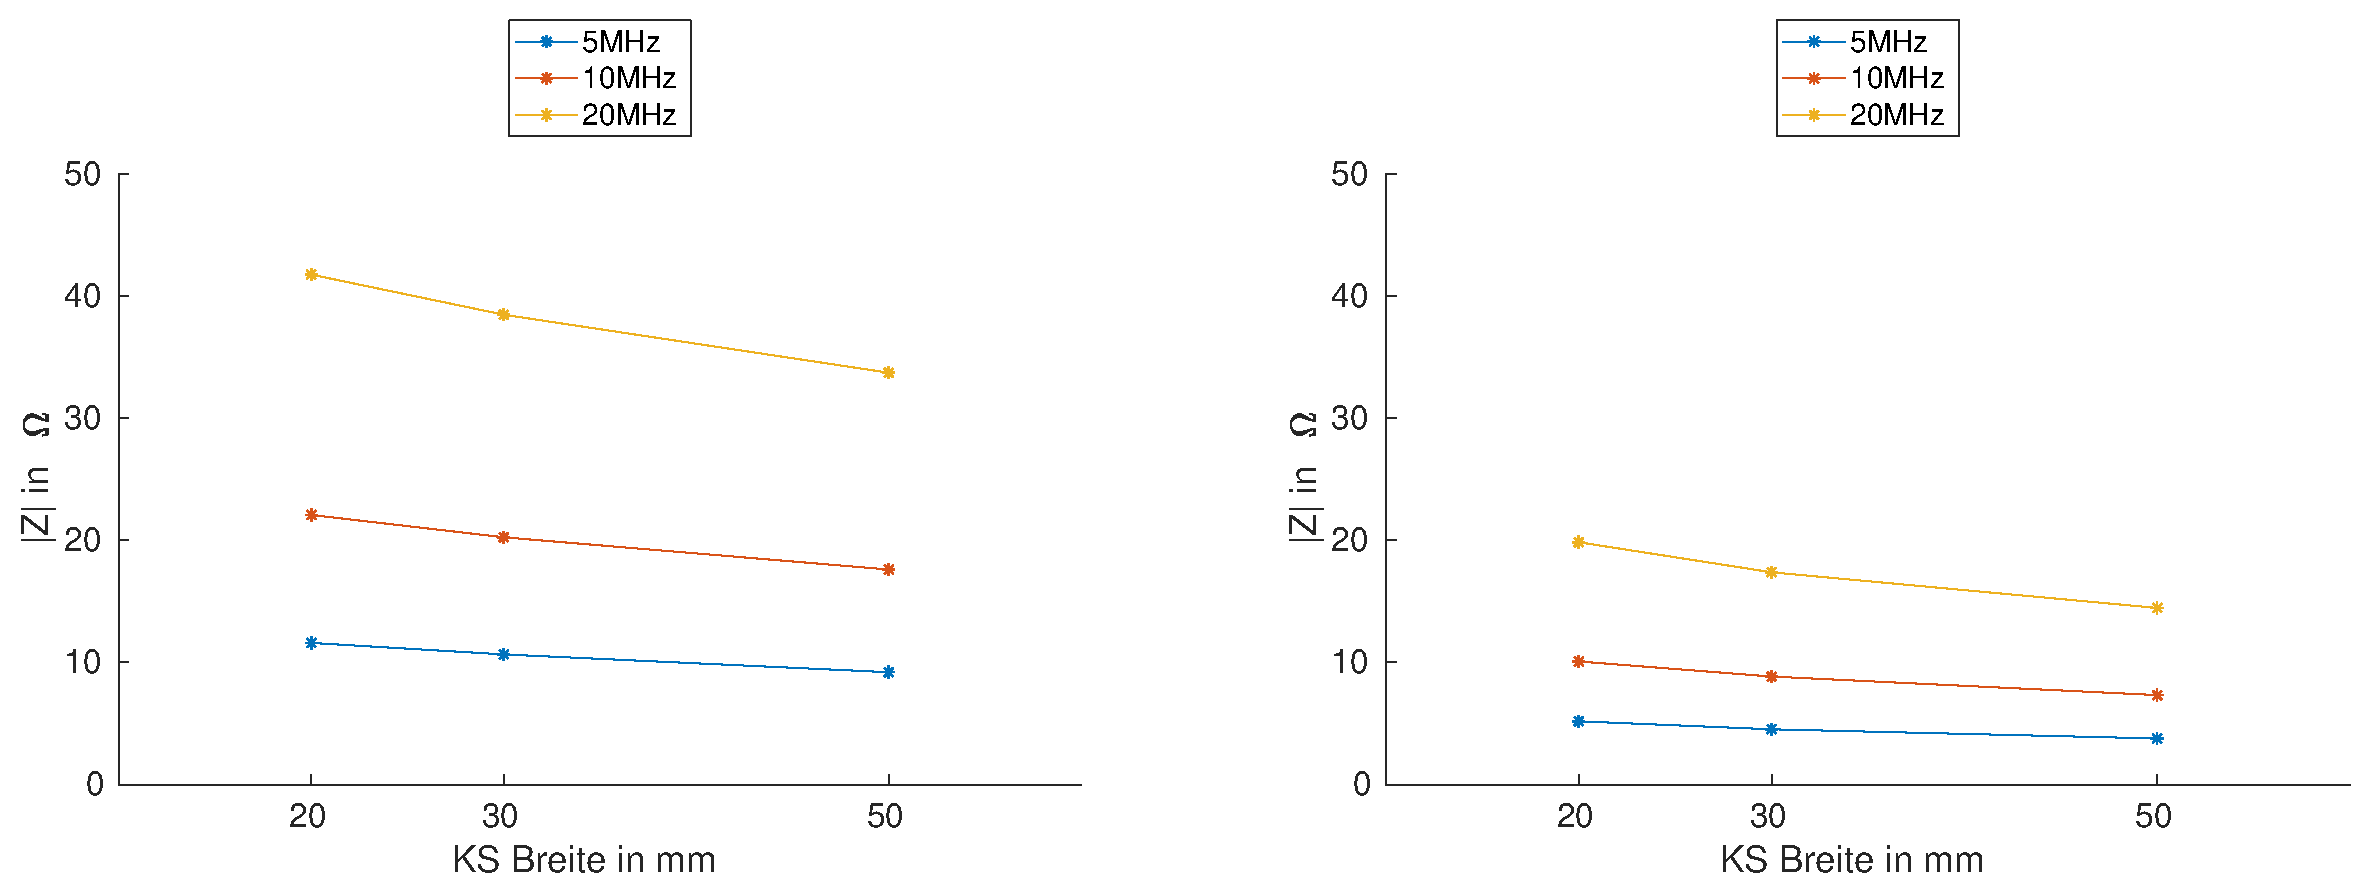
\includegraphics[width=\textwidth]{RK_Impedanz_width_frequenz}
	\caption{Gegen\"uberstellung der Ringkernimpedanz bei 5, 10 und $\SI{20}{\mega\hertz}$. Links: 1KS, rechts: 2KS.}
	\label{fig:ringcorewidth20}
\end{figure}
\par
Das Ergebnis zeigt, dass ein breiterer Kurzschluss das Ergebnis der resultierenden Ringkernimpedanz weiter verringert. Diese Variation liefert im Extremfall, also dem Unterschied von $\SI{20}{\milli\meter}$ zu $\SI{50}{\milli\meter}$ bei einer Anzahl von zwei Kurzschl\"ussen und einer Frequenz von $\SI{20}{\mega\hertz}$, eine Verringerung der Ringkernimpedanz nach Gleichung~\ref{eq:maxdiffpercent} von rund $\SI{2,8}{\%}$. Das bedeutet, dass die Breite der Kurzschl\"usse wesentlich weniger Auswirkungen auf die resultierende Ringkernimpedanz hat, wie die Anzahl an Kurzschl\"ussen. Besonders deutlich wird das im Vergleich zwischen einem Kurzschluss der Breite $\SI{50}{\milli\meter}$ mit zwei Kurzschl\"ussen der Breite $\SI{20}{\milli\meter}$. Trotz des geringeren Platzbedarfs, liefern die zwei schmalen Kurzschl\"usse eine deutlich geringere Impedanz.  Sollte aus Platzgr\"unden eine Montage breiterer Kurzschl\"usse in der Kavit\"at zu Problemen f\"uhren, so ist eine h\"ohere Anzahl von schmaleren Kurzschl\"ussen vorzuziehen. 


\subsection{L\"ange der Kurzschl\"usse}
\"Ahnlich wie die Breite ist auch die L\"ange der Kurzschl\"usse problemlos zu varrieren. Hierbei ist allerdings darauf zu achten, dass die Kurzschlussb\"ugel mit Erh\"ohung der L\"ange auch n\"aher an den Rand der Testbox, beziehungsweise der Kavit\"at heran ragen. Die getesteten verschiedenen L\"angen sind in Abbildung~\ref{fig:ringcoreheightCST} gezeigt.
\begin{figure}[htb]
	\centering
	\subfloat[$\SI{160}{\milli\meter}$]{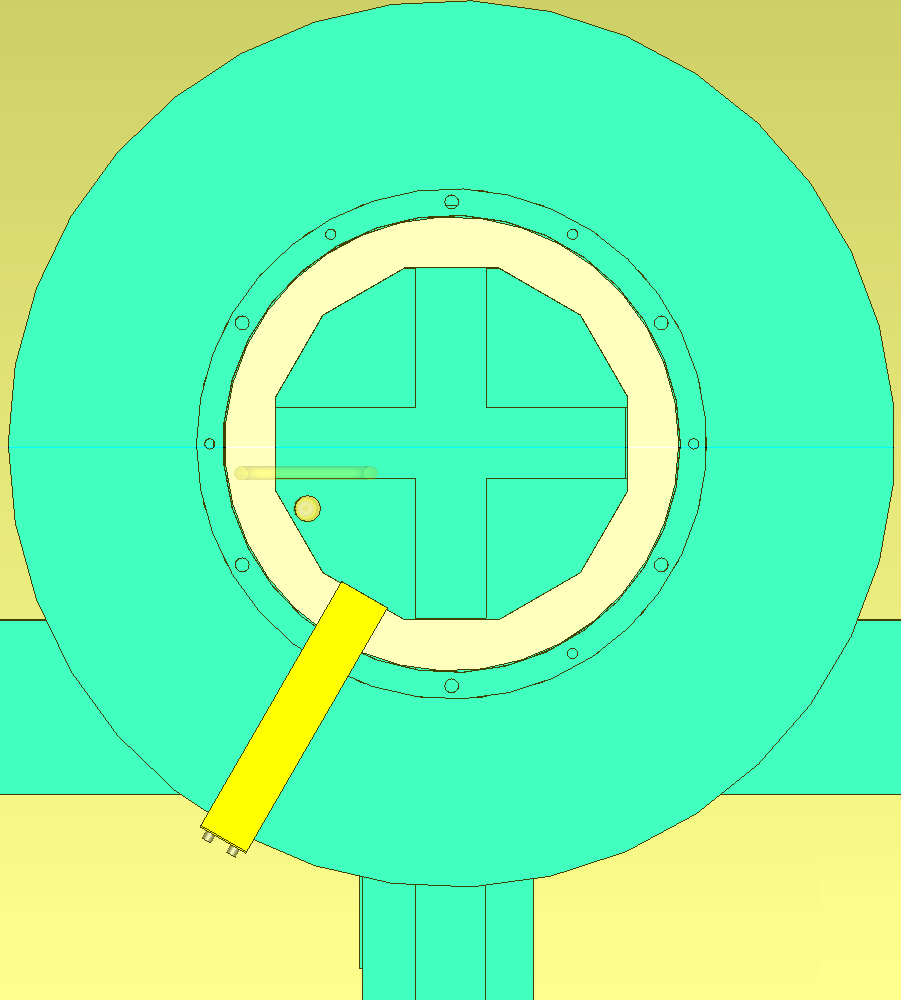
\includegraphics[height=0.3\textwidth]{1ksh160}}
	\hspace{0.05\textwidth}
	\subfloat[$\SI{200}{\milli\meter}$]{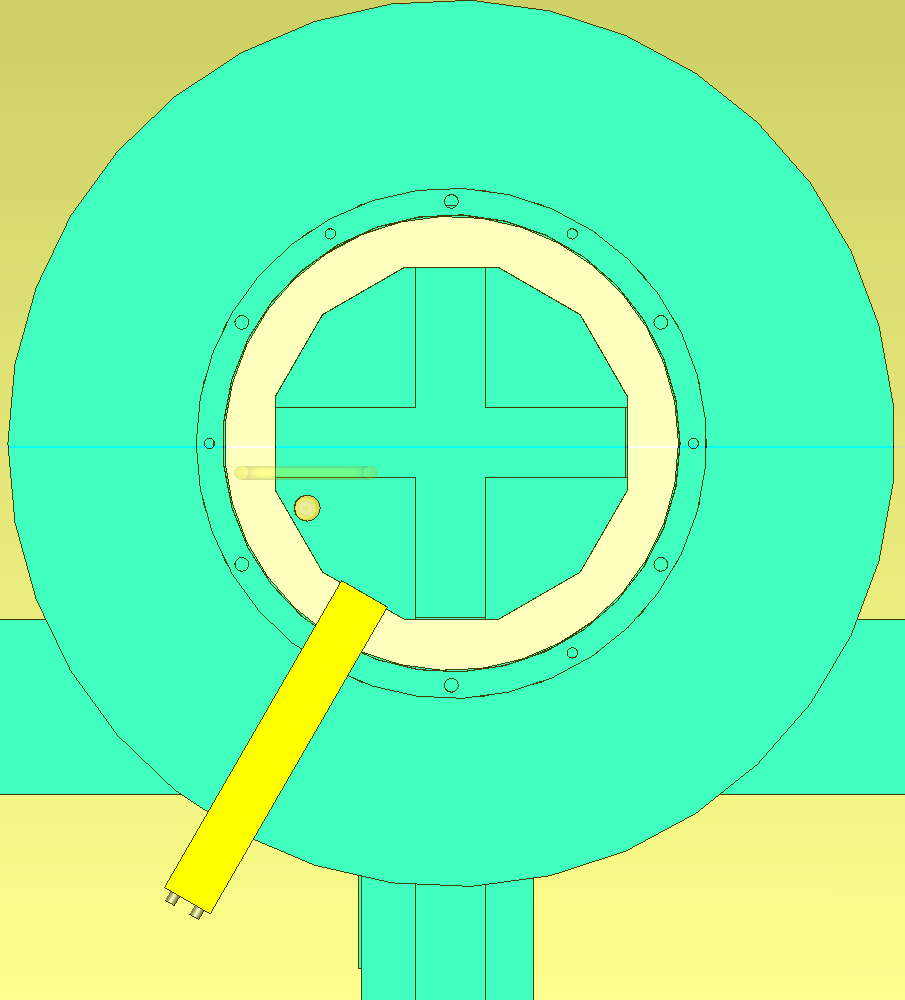
\includegraphics[height=0.3\textwidth]{1ksh200}}
	\hspace{0.05\textwidth}
	\subfloat[$\SI{250}{\milli\meter}$]{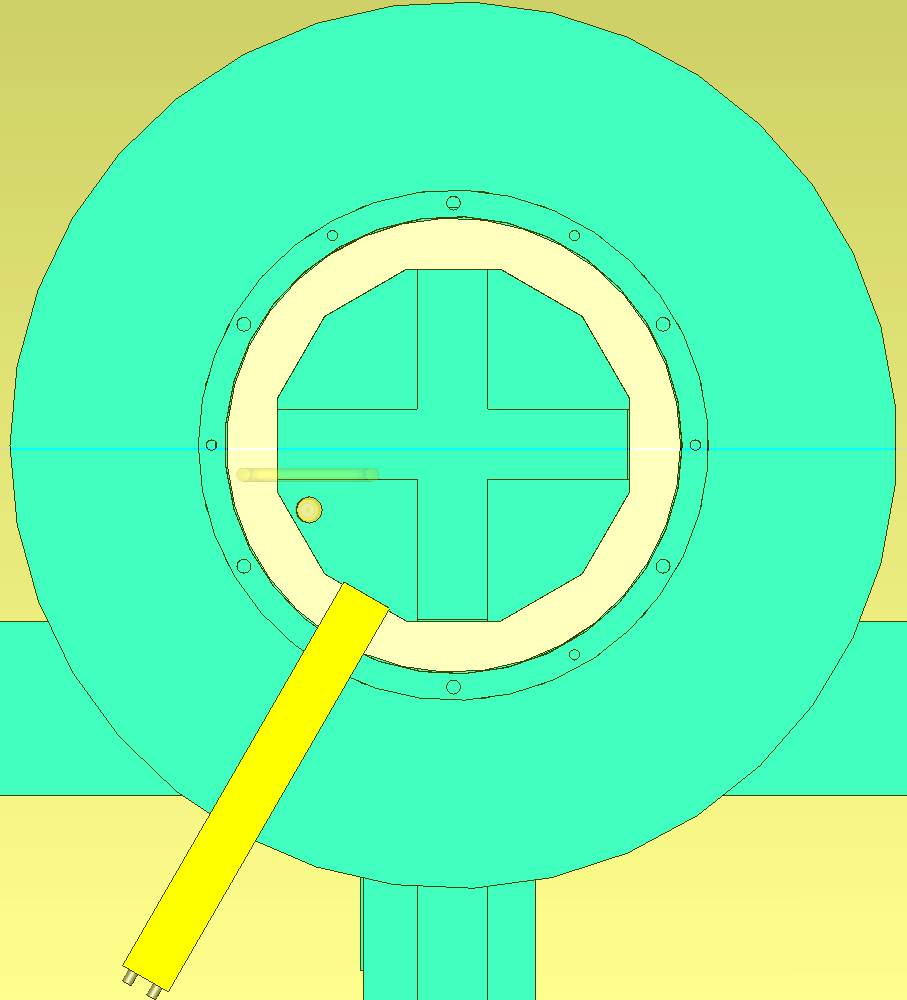
\includegraphics[height=0.3\textwidth]{1ksh250}}
	\caption{Jeweils ein montierter Kurzschluss mit verschiedenen L\"angen.}
	\label{fig:ringcoreheightCST}
\end{figure}
\par 
Die L\"ange der Kurzschl\"usse wird nach dem bekannten vorgehen analysiert. Zun\"achst wird die Ringkernimpedanz \"uber der Frequenz nach Abbildung~\ref{fig:ringcoreheight} aufgetragen.
\begin{figure}[htb]
	\centering
	\subfloat[1 Kurzschluss]{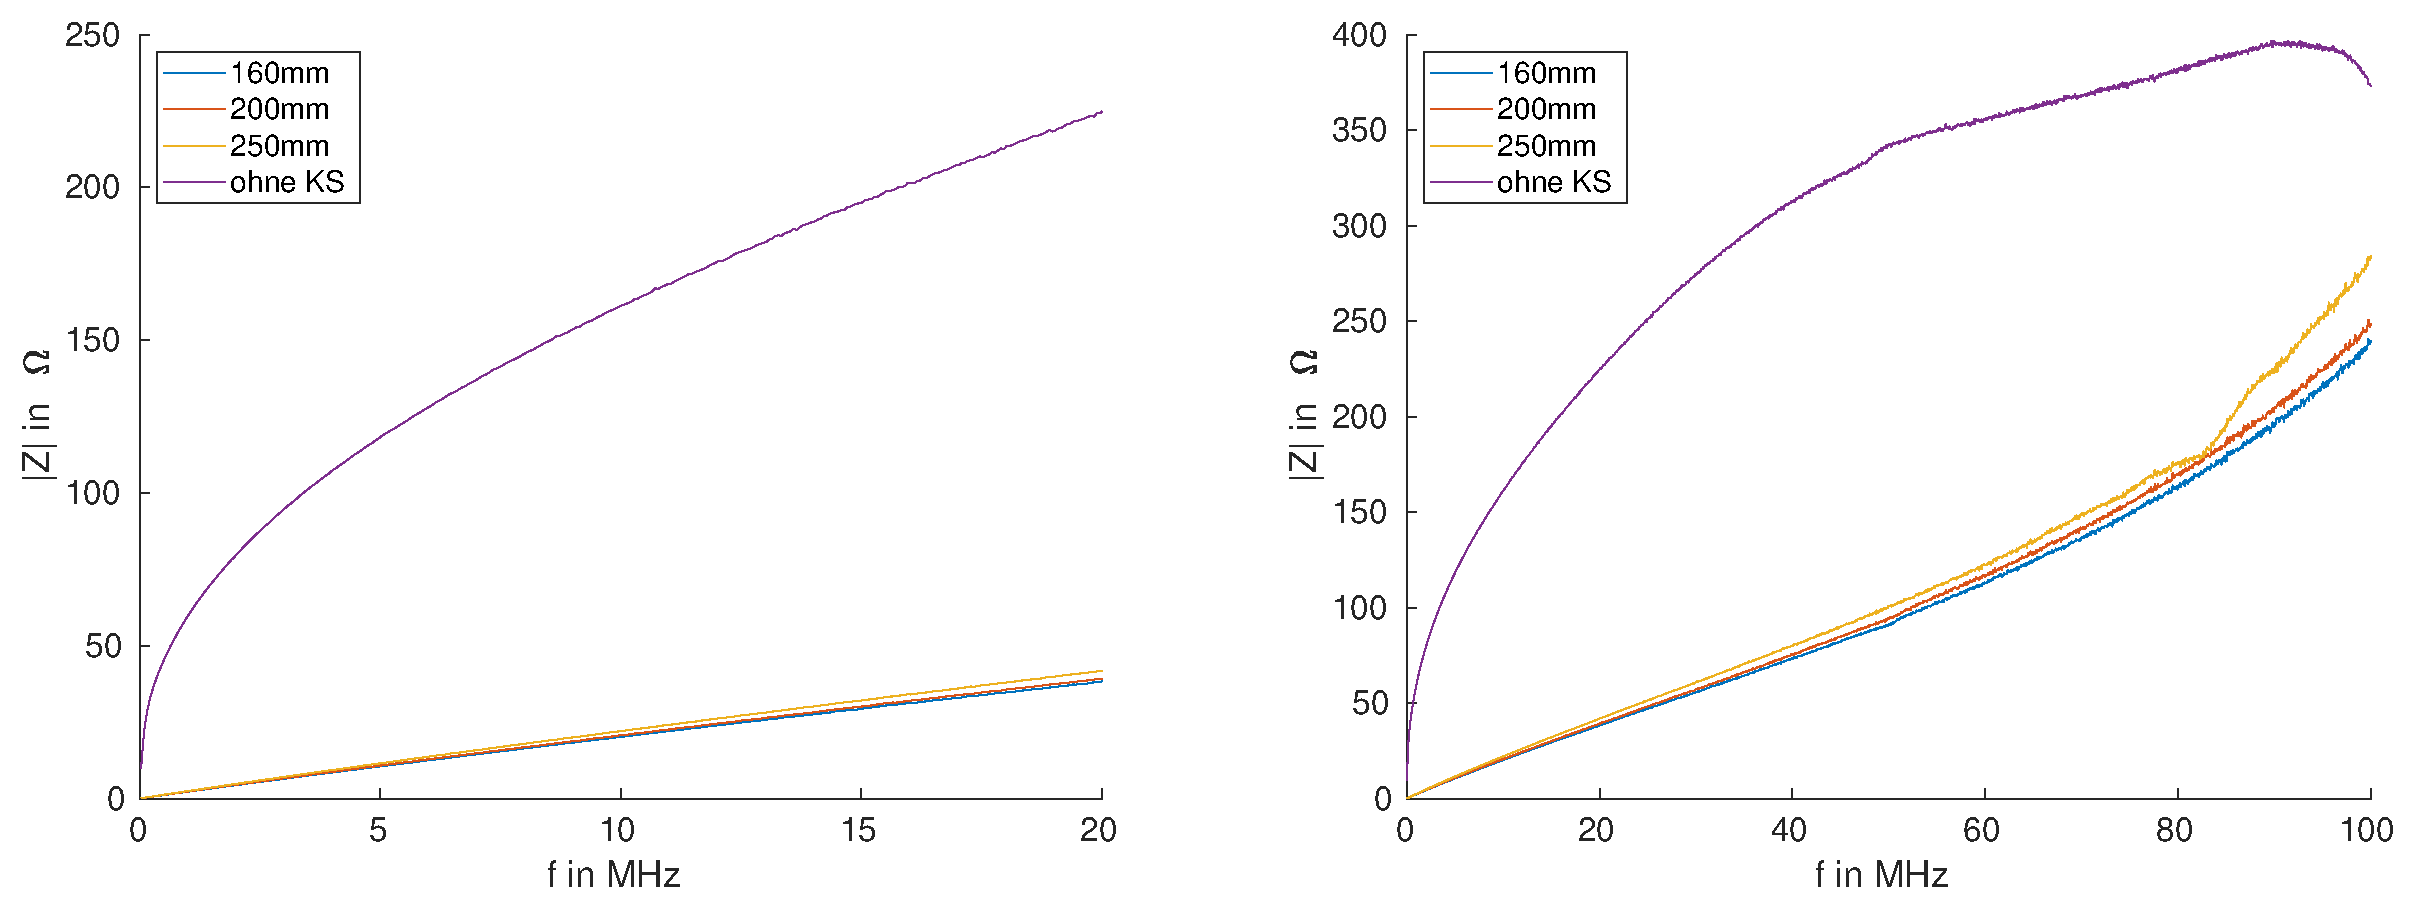
\includegraphics[width=\textwidth]{Z_RK_length_1KS}}
	\\
	\subfloat[2 Kurzschl\"usse]{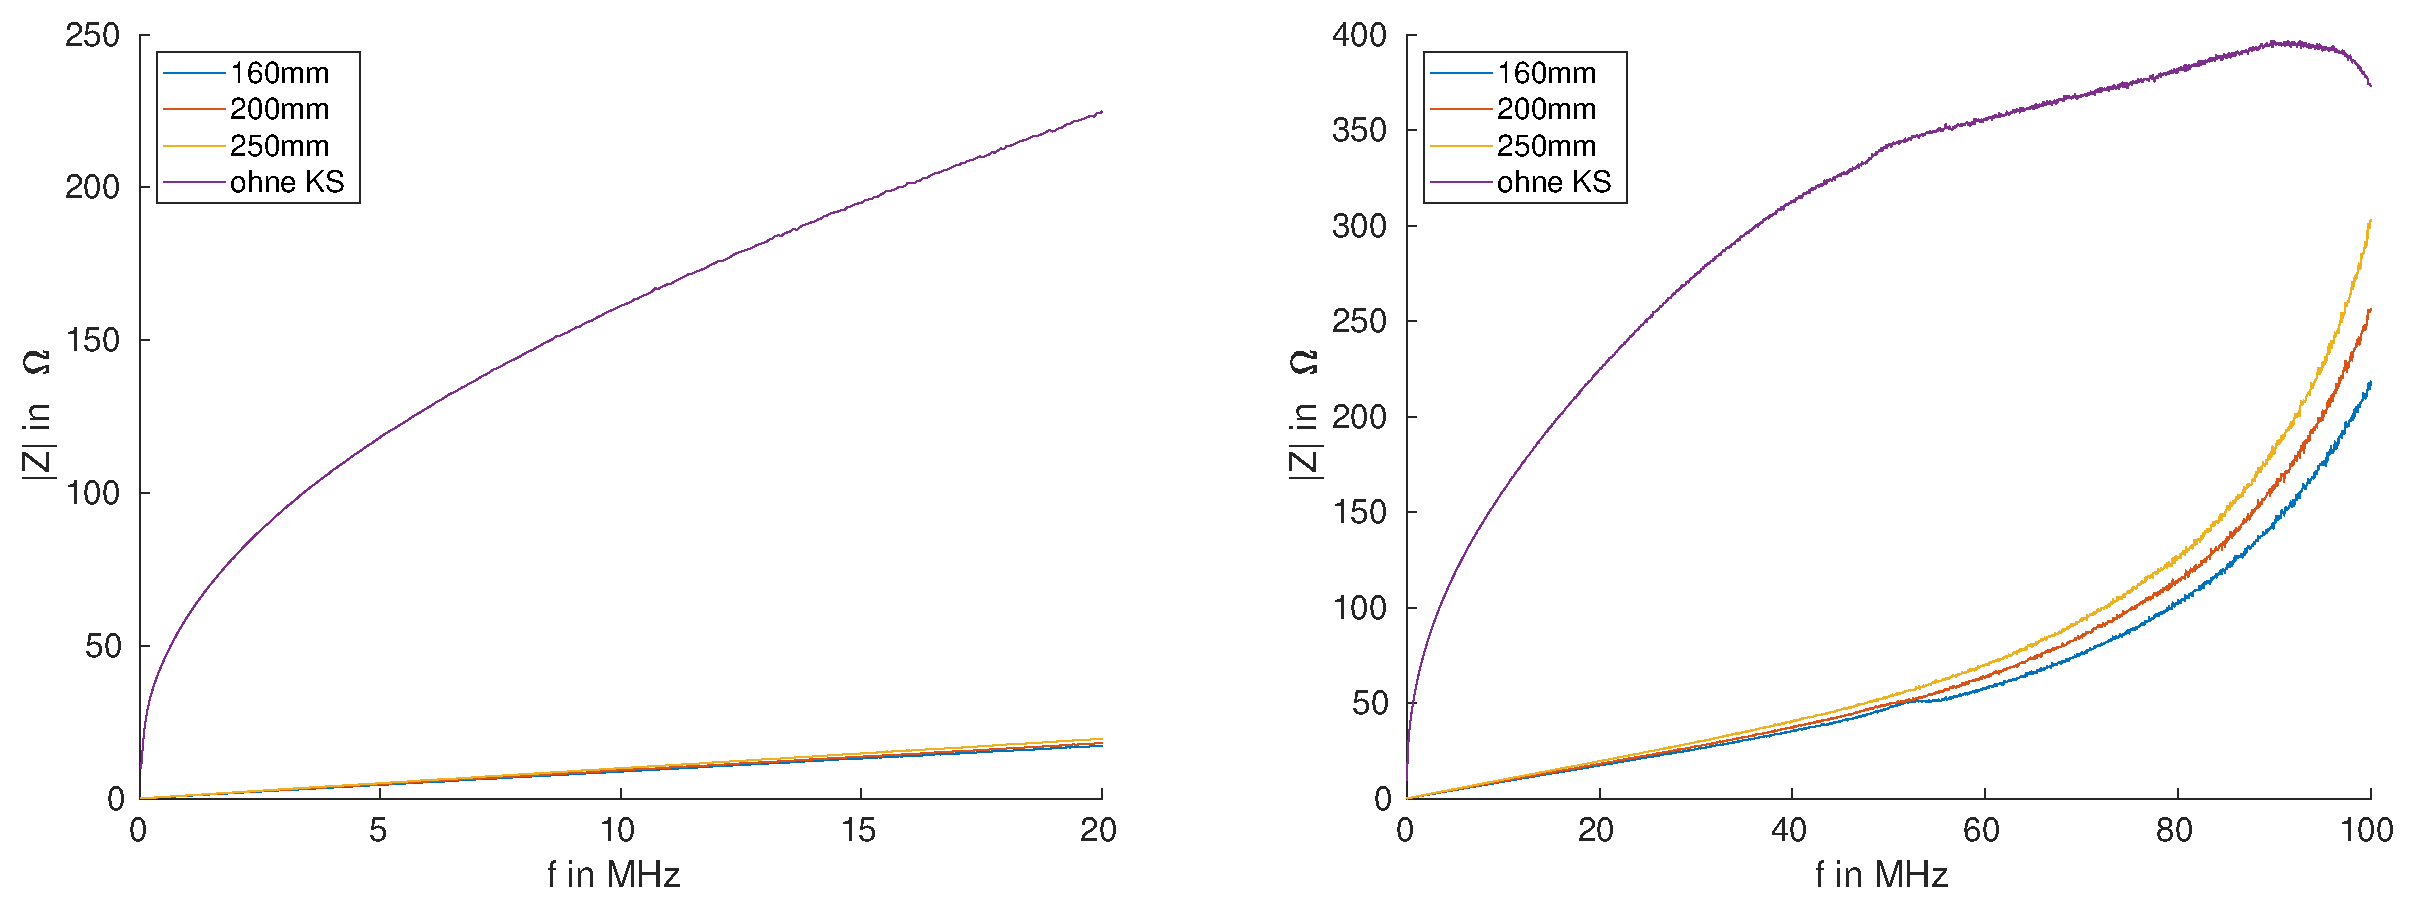
\includegraphics[width=\textwidth]{Z_RK_length_2KS}}
	\caption{Gegen\"uberstellung der Ringkernimpedanz f\"ur verschiedene L\"angen der Kurzschl\"usse.}
	\label{fig:ringcoreheight}
\end{figure}
\par
Es f\"allt auf, das der Effekt von l\"angeren Kurzschl\"ussen besonders im unteren Frequenzbereich noch deutlich geringer ausf\"allt, als bei der Breitenvariation. Um das genauer Quantifizieren zu k\"onnen werden auch hier f\"ur Frequenzen von 5, 10 und $\SI{20}{\mega\hertz}$ die Ringkernimpedanz \"uber der l\"ange der Kurzschl\"usse aufgetragen. Das Ergebnis ist in Abbildung~\ref{fig:ringcoreheight20} zu sehen.




\newpage



\begin{figure}[htb]
	\centering
	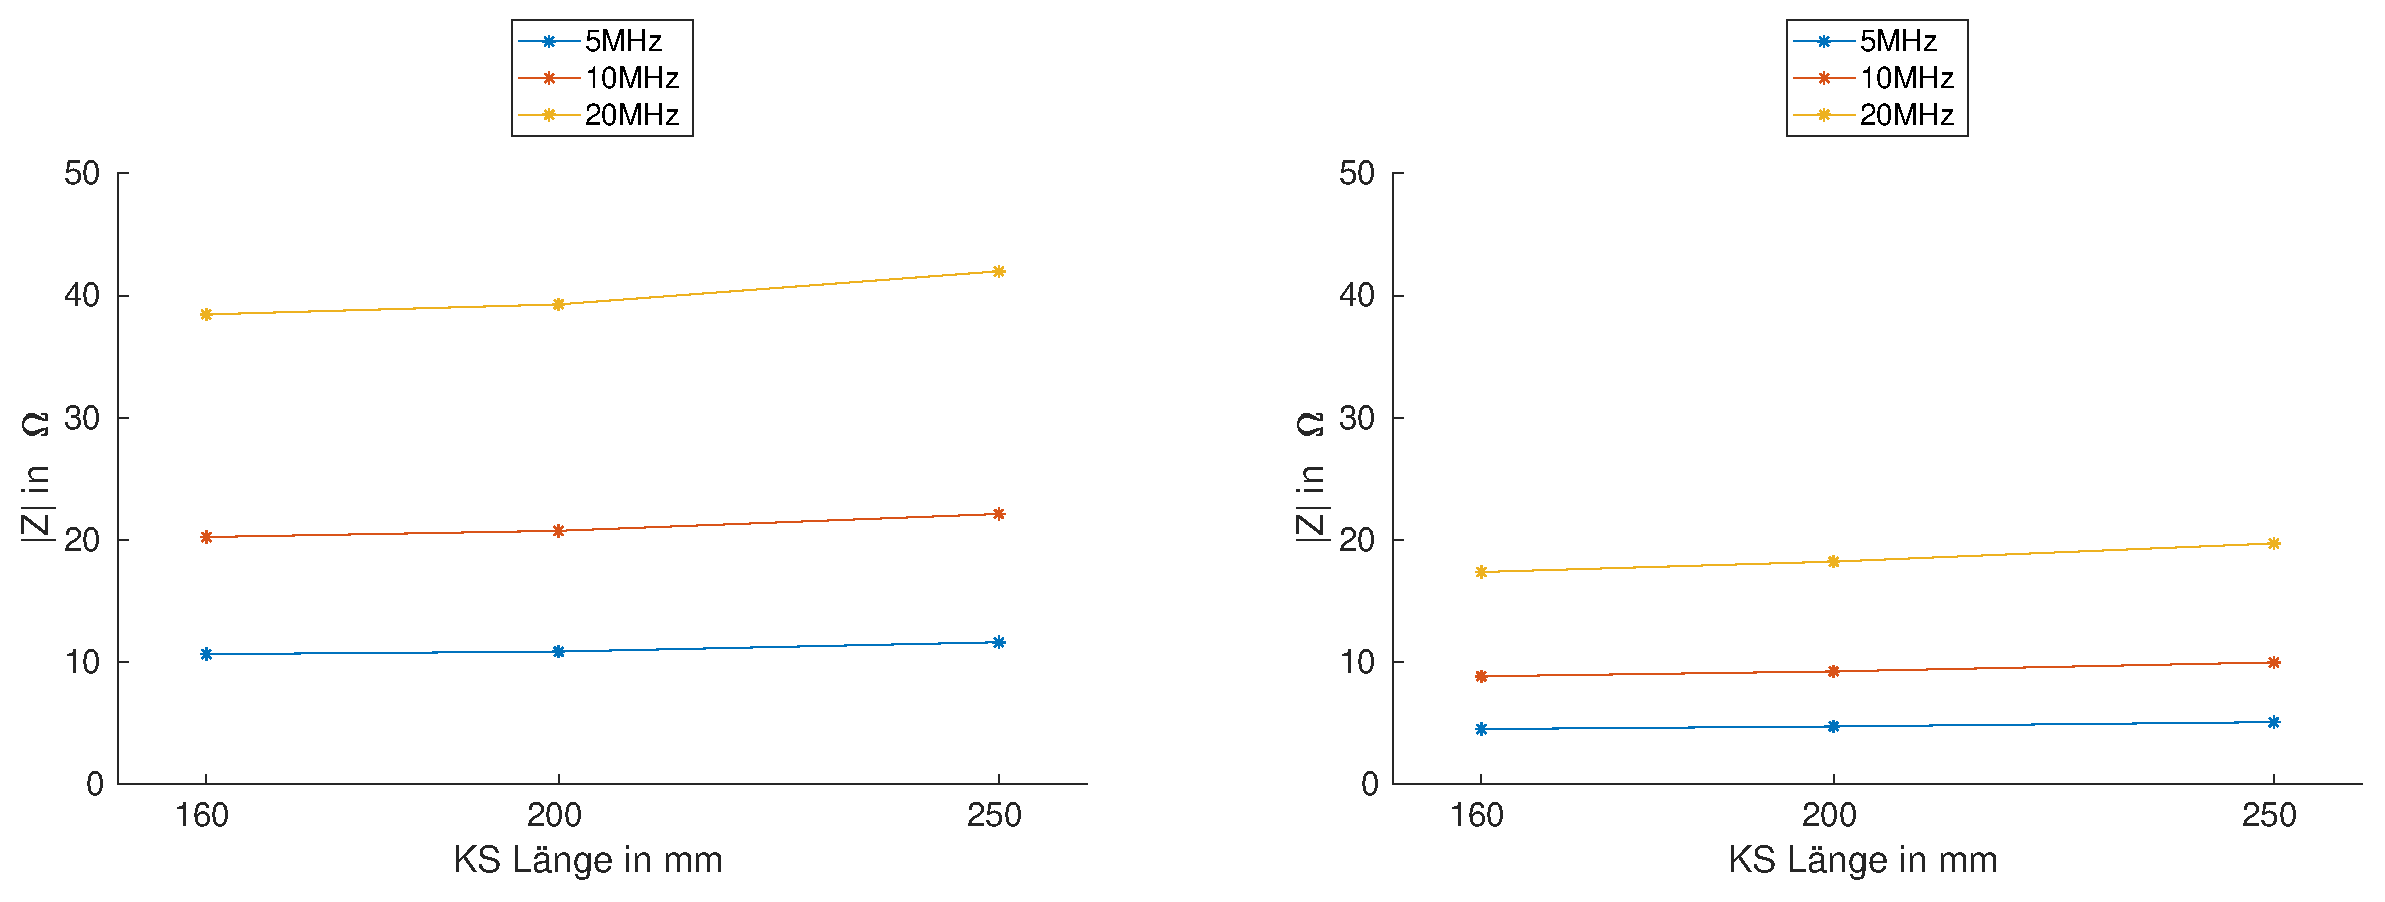
\includegraphics[width=\textwidth]{RK_Impedanz_length_frequenz}
	\caption{Gegen\"uberstellung der Ringkernimpedanz bei 5, 10 und $\SI{20}{\mega\hertz}$. Links: 1KS, rechts: 2KS.}
	\label{fig:ringcoreheight20}
\end{figure}
\par
Der Extremfall ist hier die Variation bei $\SI{20}{\mega\hertz}$ und zwei Kurzschl\"ussen zwischen $\SI{160}{\milli\meter}$ und $\SI{250}{\milli\meter}$ L\"ange. setzt man die Werte in Gleichung~\ref{eq:maxdiffpercent} ein, so erh\"alt man eine Abweichung von rund $\SI{1,3}{\%}$. 
\par
Das bedeutet, dass eine geringere L\"ange der Kurzschl\"usse bessere Ergebnisse erzeugt, und diese folglich nach M\"oglichkeit klein sein sollte. Allerdings f\"allt die Auswirkung sehr gering aus, weshalb dieser Parameter eher niedrige Priorit\"at erhalten sollte, falls der Einbau durch eine zu kleine L\"ange der Kurzschl\"usse eingeschr\"ankt wird.

\subsection{Dicke der Kurzschl\"usse}
Die Variation der Dicke ist in der Fertigung etwas aufwendiger. Zun\"achst m\"ussen die B\"ugel aus einem anderen Blech geschnitten werden. insbesondere das Biegen der B\"ugel gestaltet sich hierbei aber schwierig, da die zunehmende Dicke der Bleche das Biegen erschweren und h\"ohere Dicken anderes Werkzeug erforderten. Daher ist dieser Variationsparameter nur f\"ur zwei Dicken, n\"amlich $\SI{1}{\milli\meter}$ und $\SI{2}{\milli\meter}$ vorgesehen worden.
\par
Die Auftragung der Ringkernimpedanz \"uber der Frequenz liefert das in Abbildung~\ref{fig:ringcorethick} gezeigte Ergebnis.



\newpage




\begin{figure}[htb]
	\centering
	\subfloat[1 Kurzschluss]{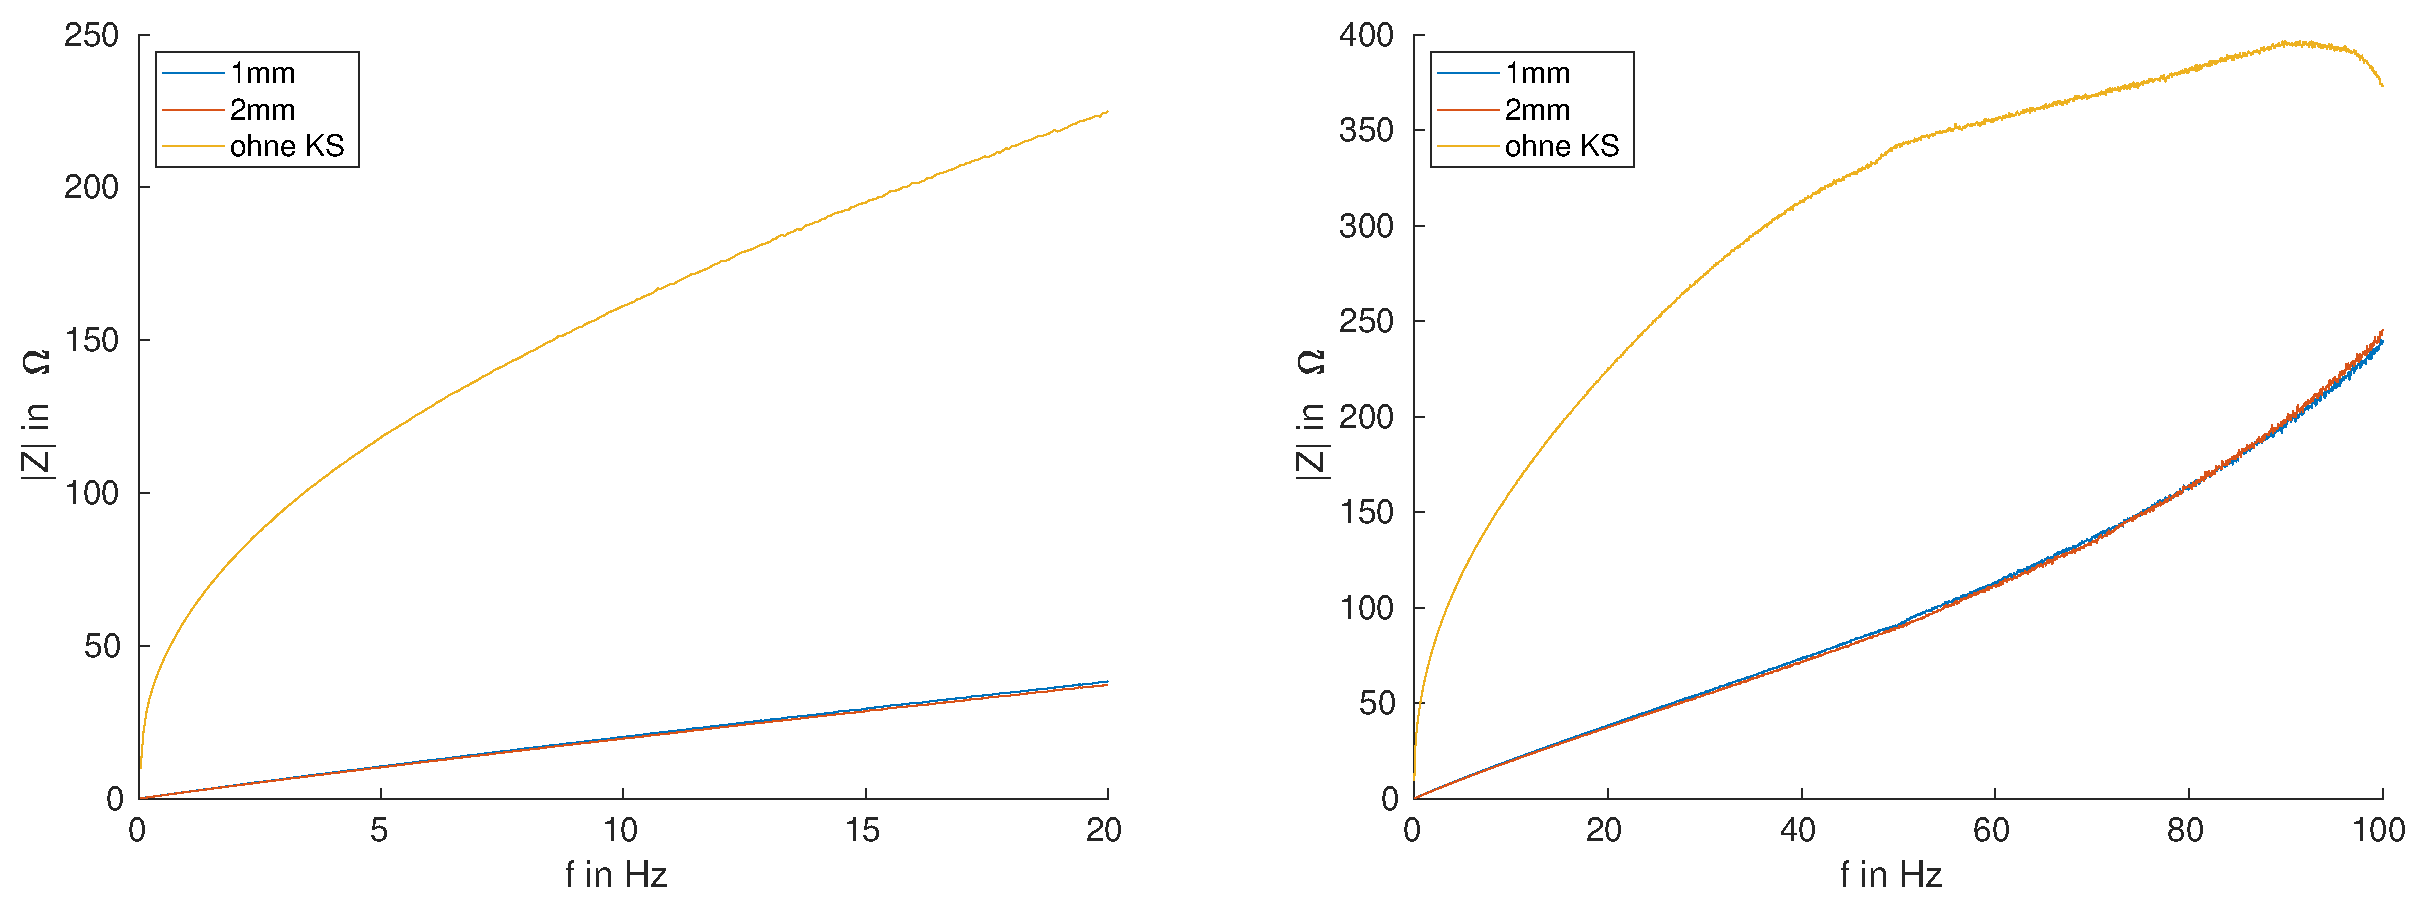
\includegraphics[width=\textwidth]{Z_RK_thick_1KS}}
	\\
	\subfloat[2 Kurzschl\"usse]{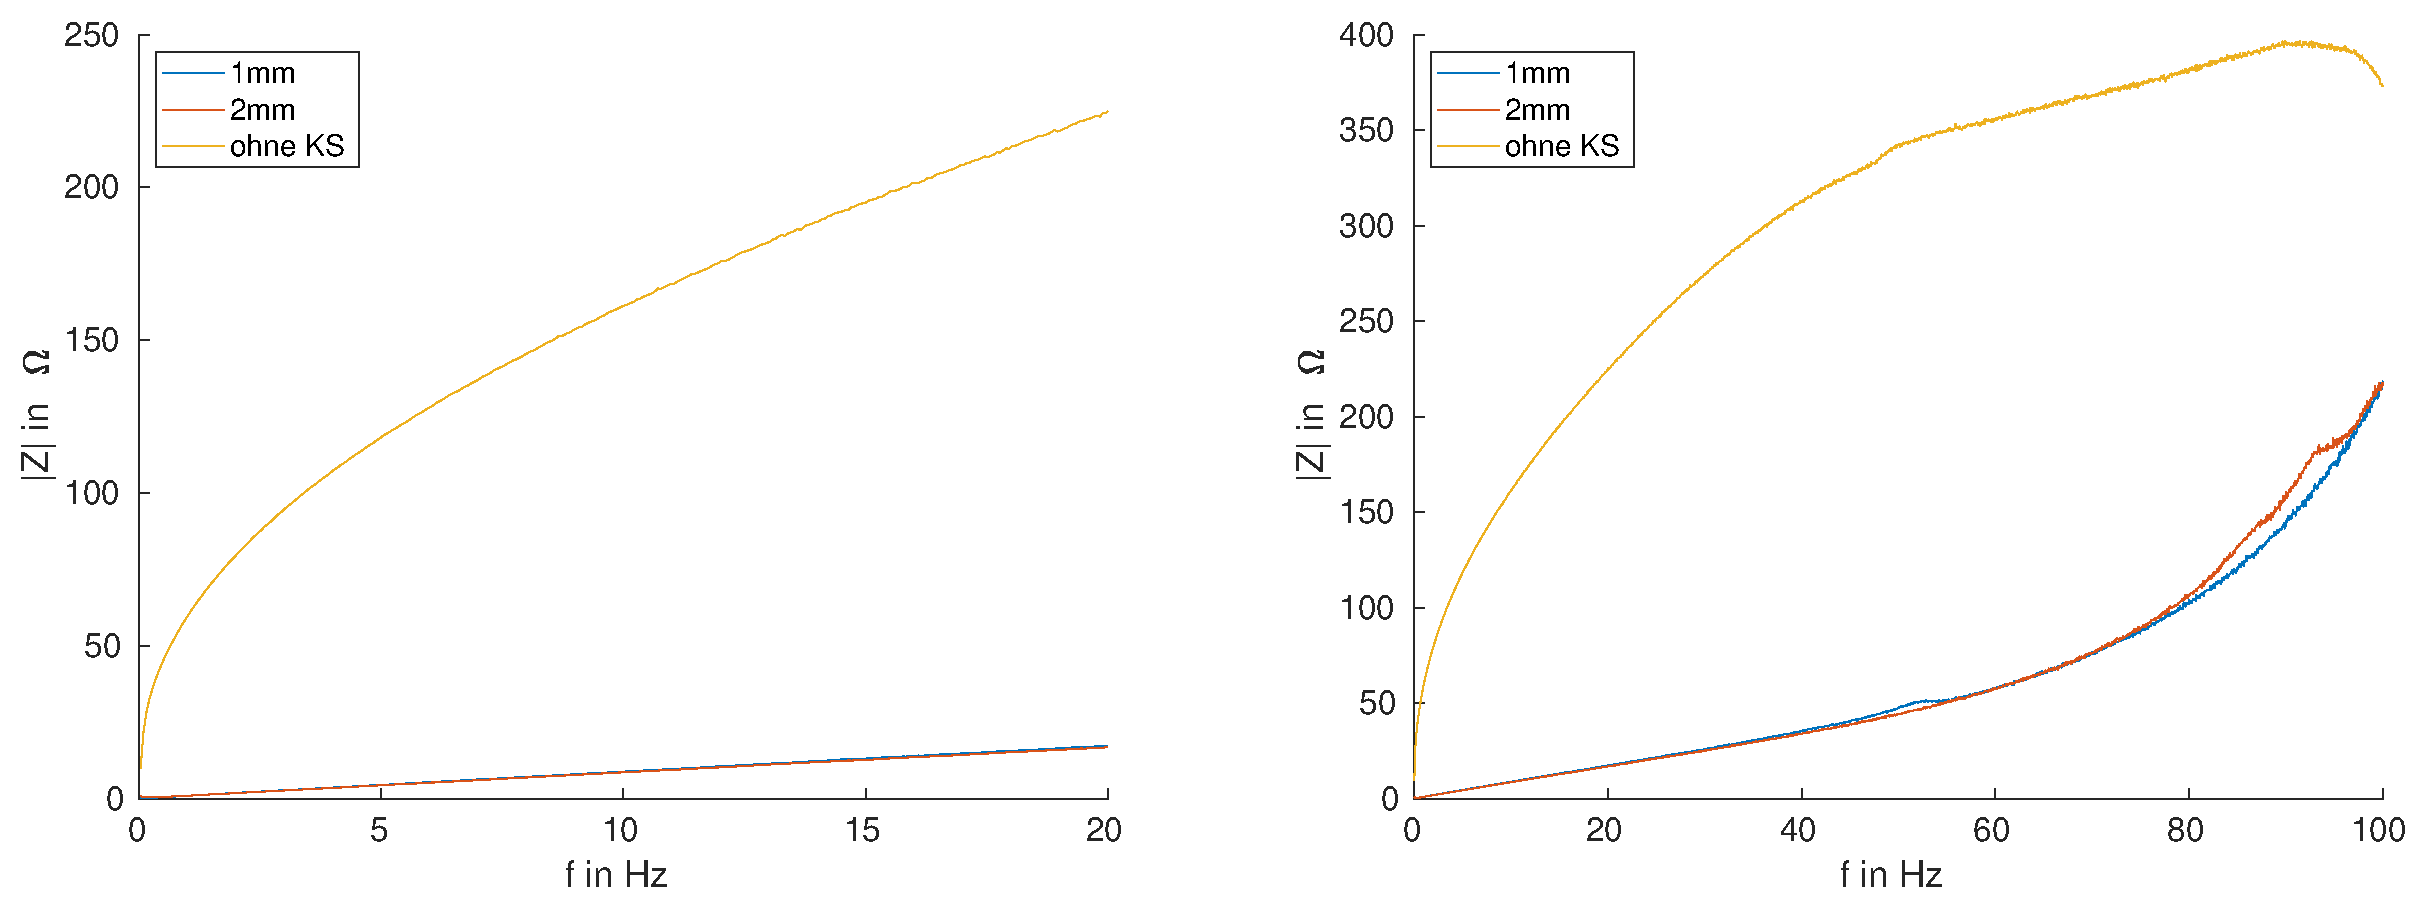
\includegraphics[width=\textwidth]{Z_RK_thick_2KS}} 
	\caption{Gegen\"uberstellung der Ringkernimpedanz f\"ur verschiedene Dicken der Kurzschl\"usse.}
	\label{fig:ringcorethick}
\end{figure}
\par
Da nur zwei Stufen f\"ur die Dicke gemessen wurden, wird in diesem Fall auf eine Grafik f\"ur die einzelnen Frequenzpunkte verzichtet. Die Berechnung der Abweichung f\"ur den Vergleich von zwei Kurzschl\"ussen bei $\SI{20}{\mega\hertz}$ mit verschiedenen Dicken liefert nach Gleichung~\ref{eq:maxdiffpercent} einen prozentualen Wert von$\SI{0,286}{\%}$. 
\par
Das bedeutet, dass die Dicke des Blechs nahezu keinen Einfluss hat.



\newpage